\documentclass{aa}  %[longauth]
\pdfoutput=1
\usepackage{graphicx}
\usepackage{txfonts}
%\usepackage{journal-macros}
\usepackage{natbib}

\bibpunct{(}{)}{;}{a}{}{,}
%%%%%%%%%%%%%%%%%%%%%%%%%%%%%%%%%%%%%%%%
%\usepackage[options]{hyperref}
% To add links in your PDF file, use the package "hyperref"
% with options according to your LaTeX or PDFLaTeX drivers.
\begin{document} 

   \title{Dissecting stellar chemical abundance space with t-SNE}

   \author{F. Anders\inst{1, 2}, C. Chiappini\inst{1, 2}, B. X. Santiago\inst{3, 2}, G. Matijevi\v{c}\inst{1}, A. B. Queiroz\inst{3, 2}, B. Barbuy\inst{4, 2}}
   
   \authorrunning{F. Anders et al.}      
   \titlerunning{t-SNE analysis of the chemistry space of the solar neighbourhood}      
   
     \institute{Leibniz-Institut f\"ur Astrophysik Potsdam (AIP), An der Sternwarte 16, 14482 Potsdam, Germany\\
              \email{fanders@aip.de}
     \and{Laborat\'orio Interinstitucional de e-Astronomia, - LIneA, Rua Gal. Jos\'e Cristino 77, Rio de Janeiro, RJ - 20921-400, Brazil}
     \and{Instituto de F\'\i sica, Universidade Federal do Rio Grande do Sul, Caixa 
Postal 15051, Porto Alegre, RS - 91501-970, Brazil}
     \and{Universidade de S\~{a}o Paulo, IAG, Rua do Mat\~{a}o 1226, Cidade Universit\'aria, 05508-900, S\~{a}o Paulo, Brazil}
	}

   \date{Received \today; accepted ...}

  \abstract
  % context heading (optional)
   {2D chemical-abundance diagrams are important diagnostics of chemo-dynamical evolution in galaxies. However, in the era of industrial Galactic astronomy opened by multi-object spectroscopic stellar surveys, the sample sizes and the number of available abundances have reached dimensions in which it has become difficult to make use of all the available information in an effective manner. Here we demonstrate the use of t-distributed stochastic neighbour embedding (t-SNE) in spectroscopic stellar abundance space of the solar vicinity. By reanalysing high-resolution high-signal-to-noise solar-neighbourhood samples with t-SNE, we find clearer chemical separations of the high- and low-[$\alpha$/Fe] disc sequences, hints for multiple populations in the high-[$\alpha$/Fe] population, and a number of chemically peculiar stars, some of which were likely born in dwarf galaxies, others possibly in the Galactic bulge.}
   \keywords{Galaxy: general -- Galaxy: abundances -- Galaxy: disk -- Galaxy: stellar content --  Stars: abundances}

   \maketitle

%________________________________________________________________

\section{Introduction}

One of the major goals of modern Galactic astrophysics is to infer the formation history of our Milky Way. To achieve this goal it is necessary to obtain precise 6D stellar kinematics as well as detailed chemical abundances for large stellar samples. This chemo-kinematical map of the Galactic stellar populations can then be compared to predictions of various Milky-Way models, eventually unveiling the star-formation and dynamical history of our Galaxy. 

Massive spectroscopic observing campaigns such as RAVE \citep{Steinmetz2006}, SEGUE \citep{Yanny2009}, APOGEE \citep{Majewski2017}, LAMOST \citep{Deng2012}, GALAH \citep{Martell2017} and the Gaia-ESO survey \citep{Gilmore2012} have in the past decade increased both the volume coverage and the statistical sample sizes by more than two orders of magnitude, to $5\cdot10^6$ stars distributed from the solar vicinity to the far side of the Galactic bulge and the outer halo. 
In spite of this recent conquista of the Milky Way in terms of number of spectroscopically analysed stars, detailed multi-abundance chemo-kinematical studies of the immediate solar vicinity \citep[e.g.]{Edvardsson1993, Fuhrmann1998, Fuhrmann2011, Fuhrmann2017, Adibekyan2012, Bensby2014, Nissen2015, Nissen2016, DelgadoMena2017} remain at least equally important for Galactic Archaeology (see \citealt{Lindegren2013} for a quantitative analysis).

The wealth of new data, especially the high dimensionality of chemo-kinematics space, requires new statistical analysis methods to efficiently constrain detailed Milky-Way formation models (including e.g. stellar evolution, stellar chemical feedback, chemical evolution, and dynamical evolution). Traditionally, the metallicity distribution function and 2D chemical-abundance diagrams ([X/Fe] vs. [Fe/H]), and abundance gradients have been used to constrain the chemical evolution of stellar populations \citep[e.g.][]{Pagel2009}. On the other hand, it is also possible to {\it define} a stellar population by chemistry (e.g. carbon-enhanced metal-poor stars - \citealt{Beers2005}; the chemical thick disc - \citealt{Gratton1996, Fuhrmann1998}; high-[$\alpha$/Fe] metal-rich stars - \citealt{Adibekyan2011}), and to then study their structural and chemo-kinematic properties in detail. This is usually done in a simple fashion, by looking at only one 2D abundance diagram. In this paper we explore the possibility of combining the information contained in various measured abundance ratios using t-distributed stochastic neighbour embedding (t-SNE) to define more robust subpopulations and better identify outliers. 

In astronomical applications, t-SNE has mainly been used to identify objects with peculiar spectra (e.g. \citealt{Matijevivc2017, Valentini2017, Traven2017, Reis2017}). 
During the writing of this paper, \citet{Kos2017} demonstrated in a complementary analysis that abundance-space t-SNE is indeed a reliable chemical-tagging tool: the authors were able to recover 7 out of 9 known open and globular clusters with high efficiency and low contamination using 13 chemical abundances from the GALAH survey \citep{Martell2017}, and they also found two new field member stars to known clusters with this technique. 

The paper is structured as follows: Sec. \ref{method} introduces t-SNE. Sections \ref{harps} and \ref{bensby} describe and discuss the results for the high-resolution spectroscopic solar-vicinity surveys of \citet{DelgadoMena2017} and \citet{Bensby2014}. We reconsider possible caveats of our results in Sec. \ref{caveats} and finish with a summary and conclusions in Sec. \ref{conclusions}.

%%%%%%%%%%%%%%%%%%%%%%%%%%%%%%%%%%%%%%%%%%%%%%%
\section{Dissecting chemistry space with t-SNE}\label{method}
%%%%%%%%%%%%%%%%%%%%%%%%%%%%%%%%%%%%%%%%%%%%%%%

Interpreting the multi-dimensional abundance distributions determined by spectroscopic surveys is not a trivial task, since different abundance diagrams contain different nucleosynthetic information and may be affected by different observational errors. A convenient way to simplify this problem is dimensionality reduction, i.e. the projection of the N-dimensional abundance space onto a lower-dimensional space in which the chemical similarity between two stars is reflected by their distance in that space. Possibly the best-known such method is called principal component analysis (PCA), widely used also in astronomical literature. For highly-correlated datasets such as spectral pixel spaces or chemical-abundance spaces, however, more sophisticated non-linear methods like IsoMap or locally linear embedding are known to perform much better \citep[e.g.][]{Matijevivc2012, Ivezic2013}.

In this paper, we reanalyse the high-resolution spectroscopic solar-vicinity surveys of \citet{Bensby2014} and \citet{DelgadoMena2017} using a machine-learning algorithm called t-distributed stochastic neighbour embedding \citep[t-SNE;][]{Hinton2003, vanderMaaten2008}. This method is widely used in big-data analytics, and is able to efficiently project complex datasets onto a 2D plane in which the proximity between similar data points is preserved. We use the python implementation of t-SNE included in the {\tt scikit-learn} package \citep{Pedregosa2012} and refer to the original papers and the online documentation for details about the method and code. In short, the advantage of using t-SNE over other manifold-learning techniques is that it performs much better in revealing structure at many different scales \citep{vanderMaaten2008, Matijevivc2017}, which is a necessary feature when looking for chemical substructure in the Galactic disc.

{\it How t-SNE works:} For a given set of $N$ high-dimensional datapoints $\mathbf{x}_1, \dots, \mathbf{x}_N$ (images, spectra, or in our case chemical-abundance vectors), t-SNE first computes pairwise similarity probabilities $p_{ij}$ for the points $\mathbf{x}_i$ and $\mathbf{x}_j$:
$$p_{j\mid i} = \frac{\exp(-\lVert\mathbf{x}_i - \mathbf{x}_j\rVert^2 / 2\sigma_i^2)}{\sum_{k \neq i} \exp(-\lVert\mathbf{x}_i - \mathbf{x}_k\rVert^2 / 2\sigma_i^2)}.$$
To circumvent problems with outliers, the symmetrised similarity of $x_j$ and $x_i$ is defined as 
$$p_{ij} = \frac{p_{j\mid i} + p_{i\mid j}}{2N}.$$

In the next step, t-SNE attepts to learn a $d$-dimensional map $\mathbf{y}_1, \dots, \mathbf{y}_N$ (in general $d=2$) that reflects the similarities  $p_{ij}$ similarities between two points $\mathbf{y}_i$ and $\mathbf{y}_j$ in the low-dimensional map, defined as
$$q_{ij} = \frac{(1 + \lVert \mathbf{y}_i - \mathbf{y}_j\rVert^2)^{-1}}{\sum_{k \neq m} (1 + \lVert \mathbf{y}_k - \mathbf{y}_m\rVert^2)^{-1}}.$$
This metric uses Student's $t$ distribution to avoid crowding problems in the low-dimensional map \citep{vanderMaaten2008}. Starting from a random Gaussian distribution in the $d$-dimensional map, the locations of the points $\mathbf{y}_i$ are determined by minimizing the Kullback–Leibler divergence \citep{Kullback1951} between the low- and high-dimensional similarity distributions $Q$ and $P$:
$$KL(P||Q) = \sum_{i \neq j} p_{ij} \log \frac{p_{ij}}{q_{ij}},$$
using a gradient-descent method. The result of this optimization is a 2D (or 3D) map that reflects the similarities between the high-dimensional inputs (see e.g. Fig. \ref{harps1}).

The method has one main parameter, the so-called perplexity, $p$, which governs the bandwidth of the Gaussian kernels $\sigma_i$ appearing in the similarities $p_{ij}$. As a result, the bandwidth is adapted to the density of the data: smaller values of $\sigma_i$ are used in denser parts of the data space. The perplexity parameter can be thought of as a guess about the number of close neighbors each point has, and therefore the ideal value for $p$ depends on the sample size. A change in perplexity has in many cases a complex effect on the resulting map, and different values for $p$ should be explored \citep{Wattenberg2016}. 

Recently, \citet{Linderman2017} demonstrated that two other hyper-parameters of t-SNE can be chosen optimally: the learning rate should be set to $\sim 1$, and the early-exaggeration parameter should be set to $\sim 0.1$ times the sample size. In the following, we use these recommendations.

In addition, t-SNE, as a genuine machine-learning technique, does have two drawbacks that are relevant for our science case. First, it does not account for individual uncertainties, and may therefore be affected by extremely heteroscedastic errors. Secondly, its current implementations do not allow to treat missing data, so that any star with a missing individual abundance measurement has to be excluded. 

%%%%%%%%%%%%%%%%%%%%%%%%%%%%%%%%%%%%%%%%%%%%%%%
\section{Re-analysing the HARPS GTO sample}\label{harps}
%%%%%%%%%%%%%%%%%%%%%%%%%%%%%%%%%%%%%%%%%%%%%%%

\begin{figure*}\centering
%\sidecaption
 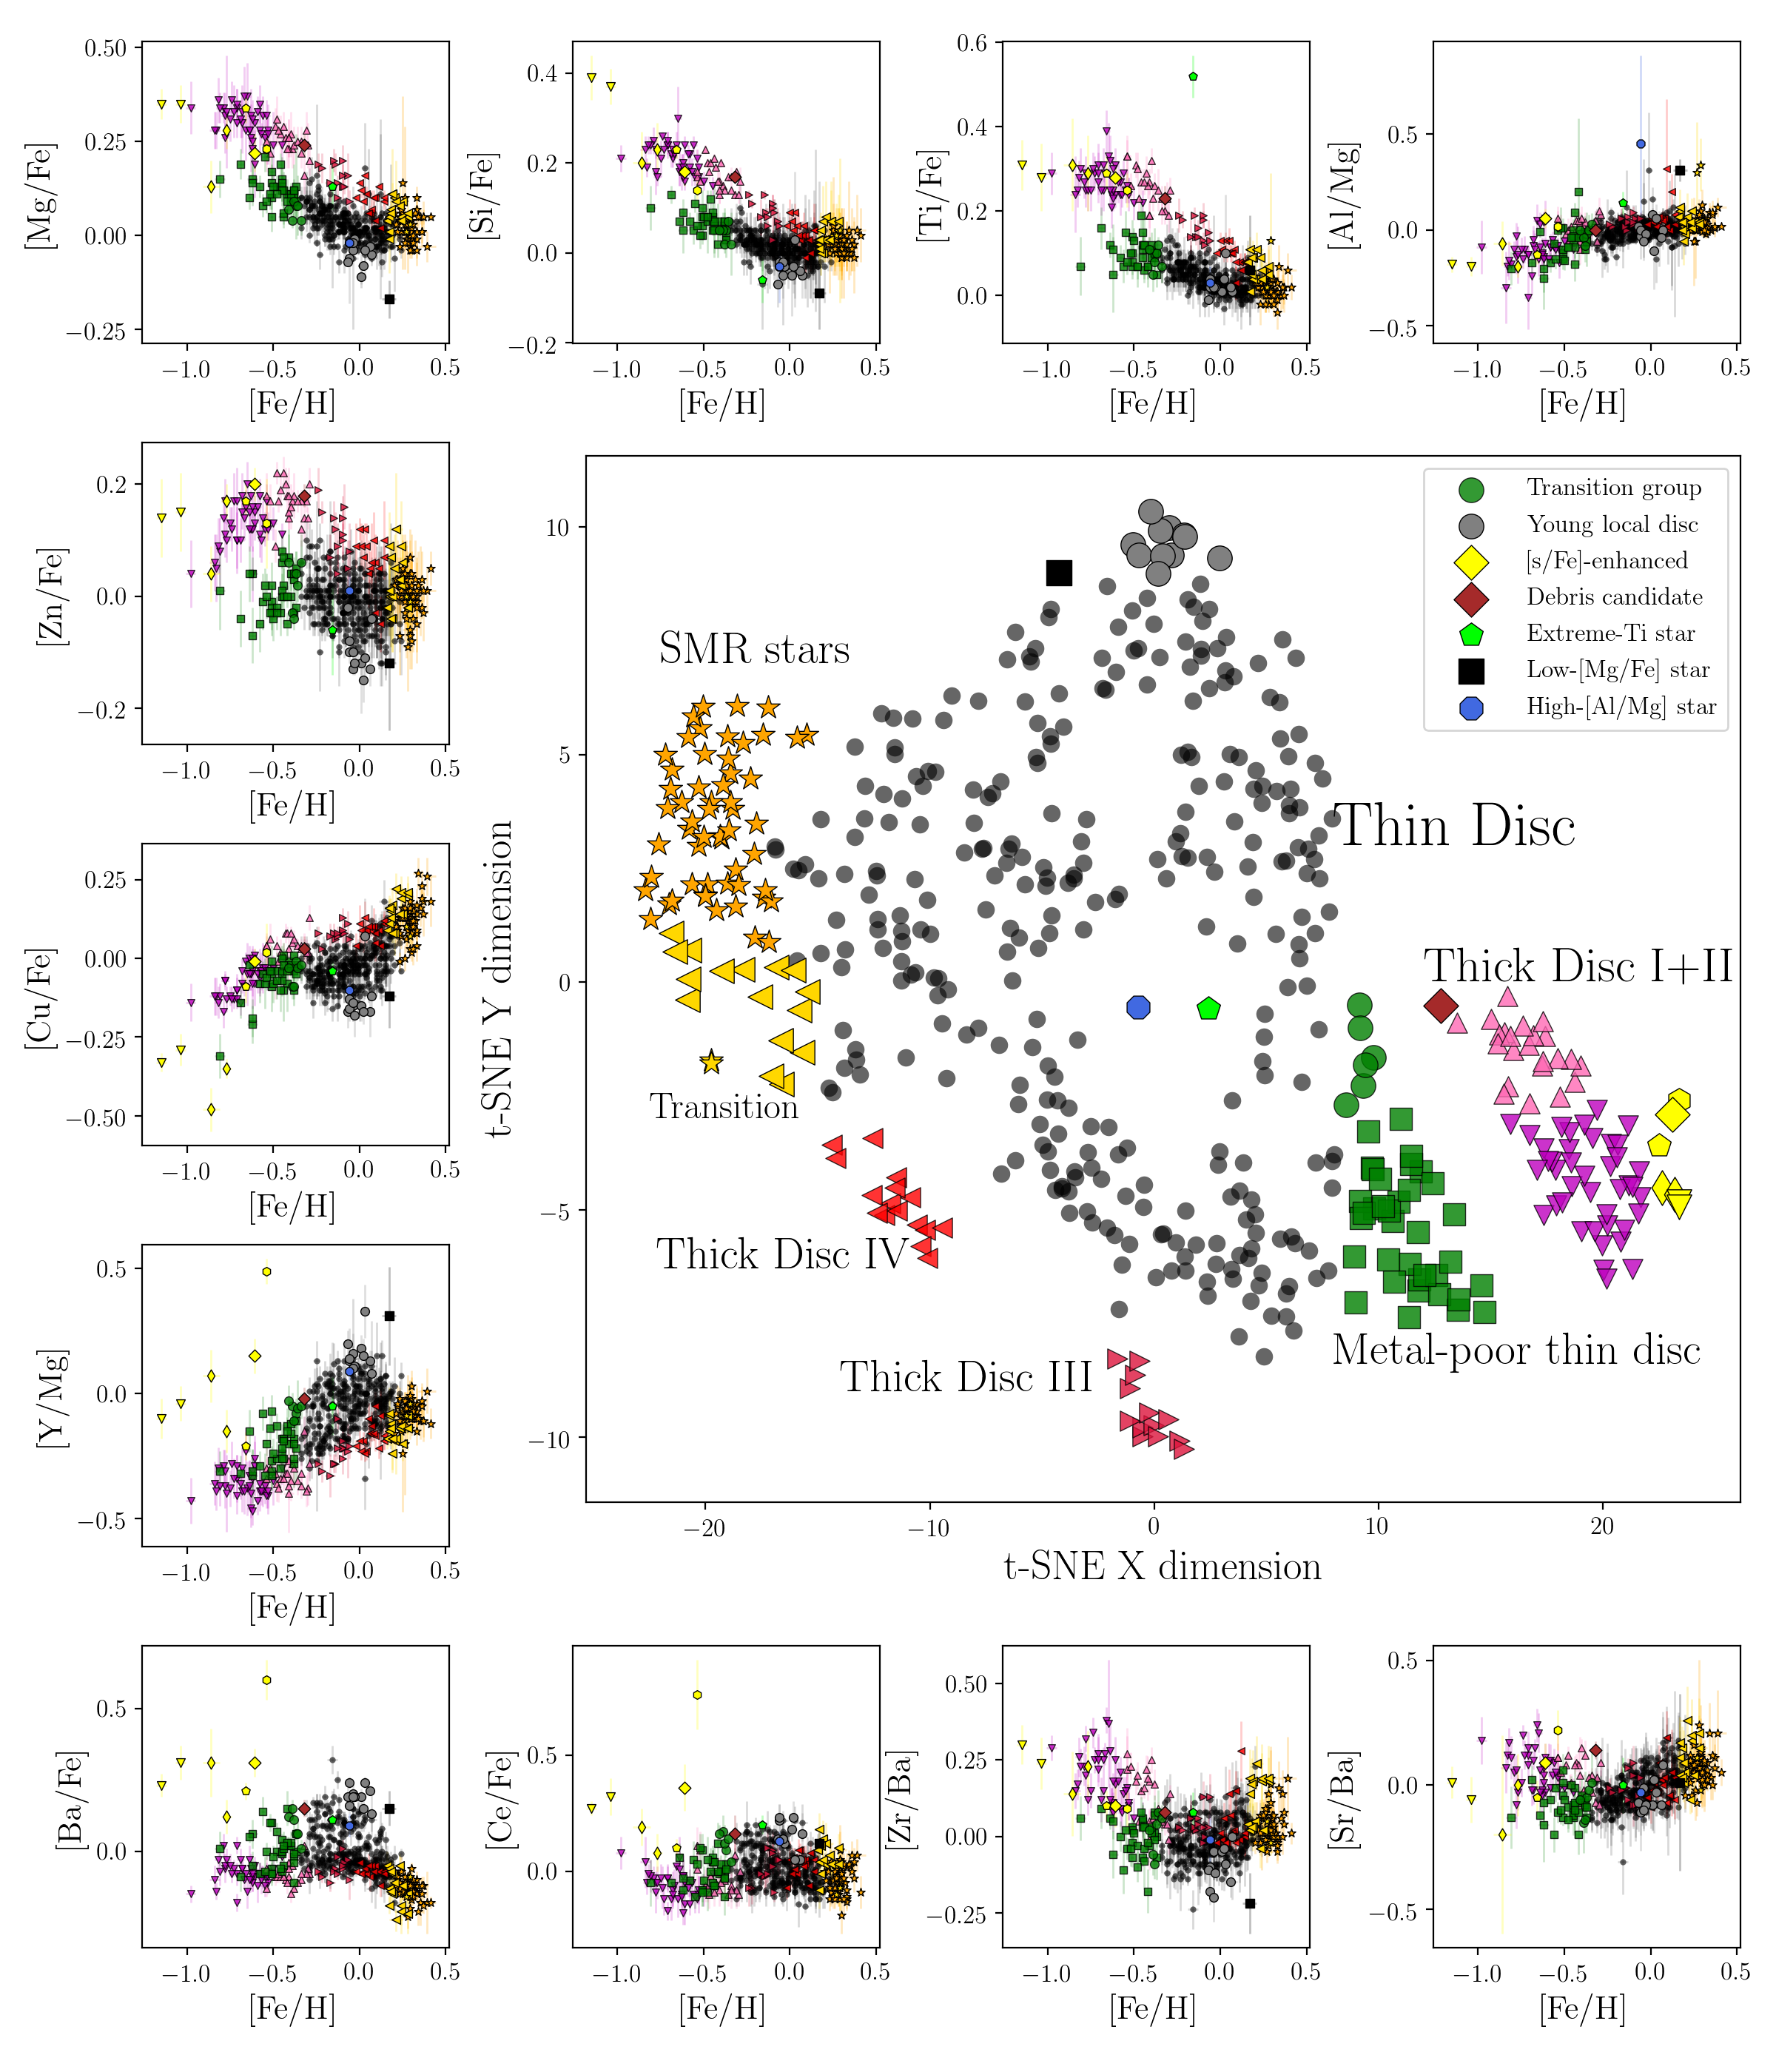
\includegraphics[width=0.8\textwidth]{im/harps_tsne-abundsplot_teffcut.png}
\caption{Illustration of how t-SNE works in abundance space, using the \citet{DelgadoMena2017} sample. The small panels show eleven of the possible $\sim20,000$ abundance diagrams that can be created from 13 elements. The resulting reference t-SNE projection of the full abundance space is shown in the big panel, and several identified subgroups are indicated.}
\label{harps0}
\end{figure*}

\begin{figure*}\centering
 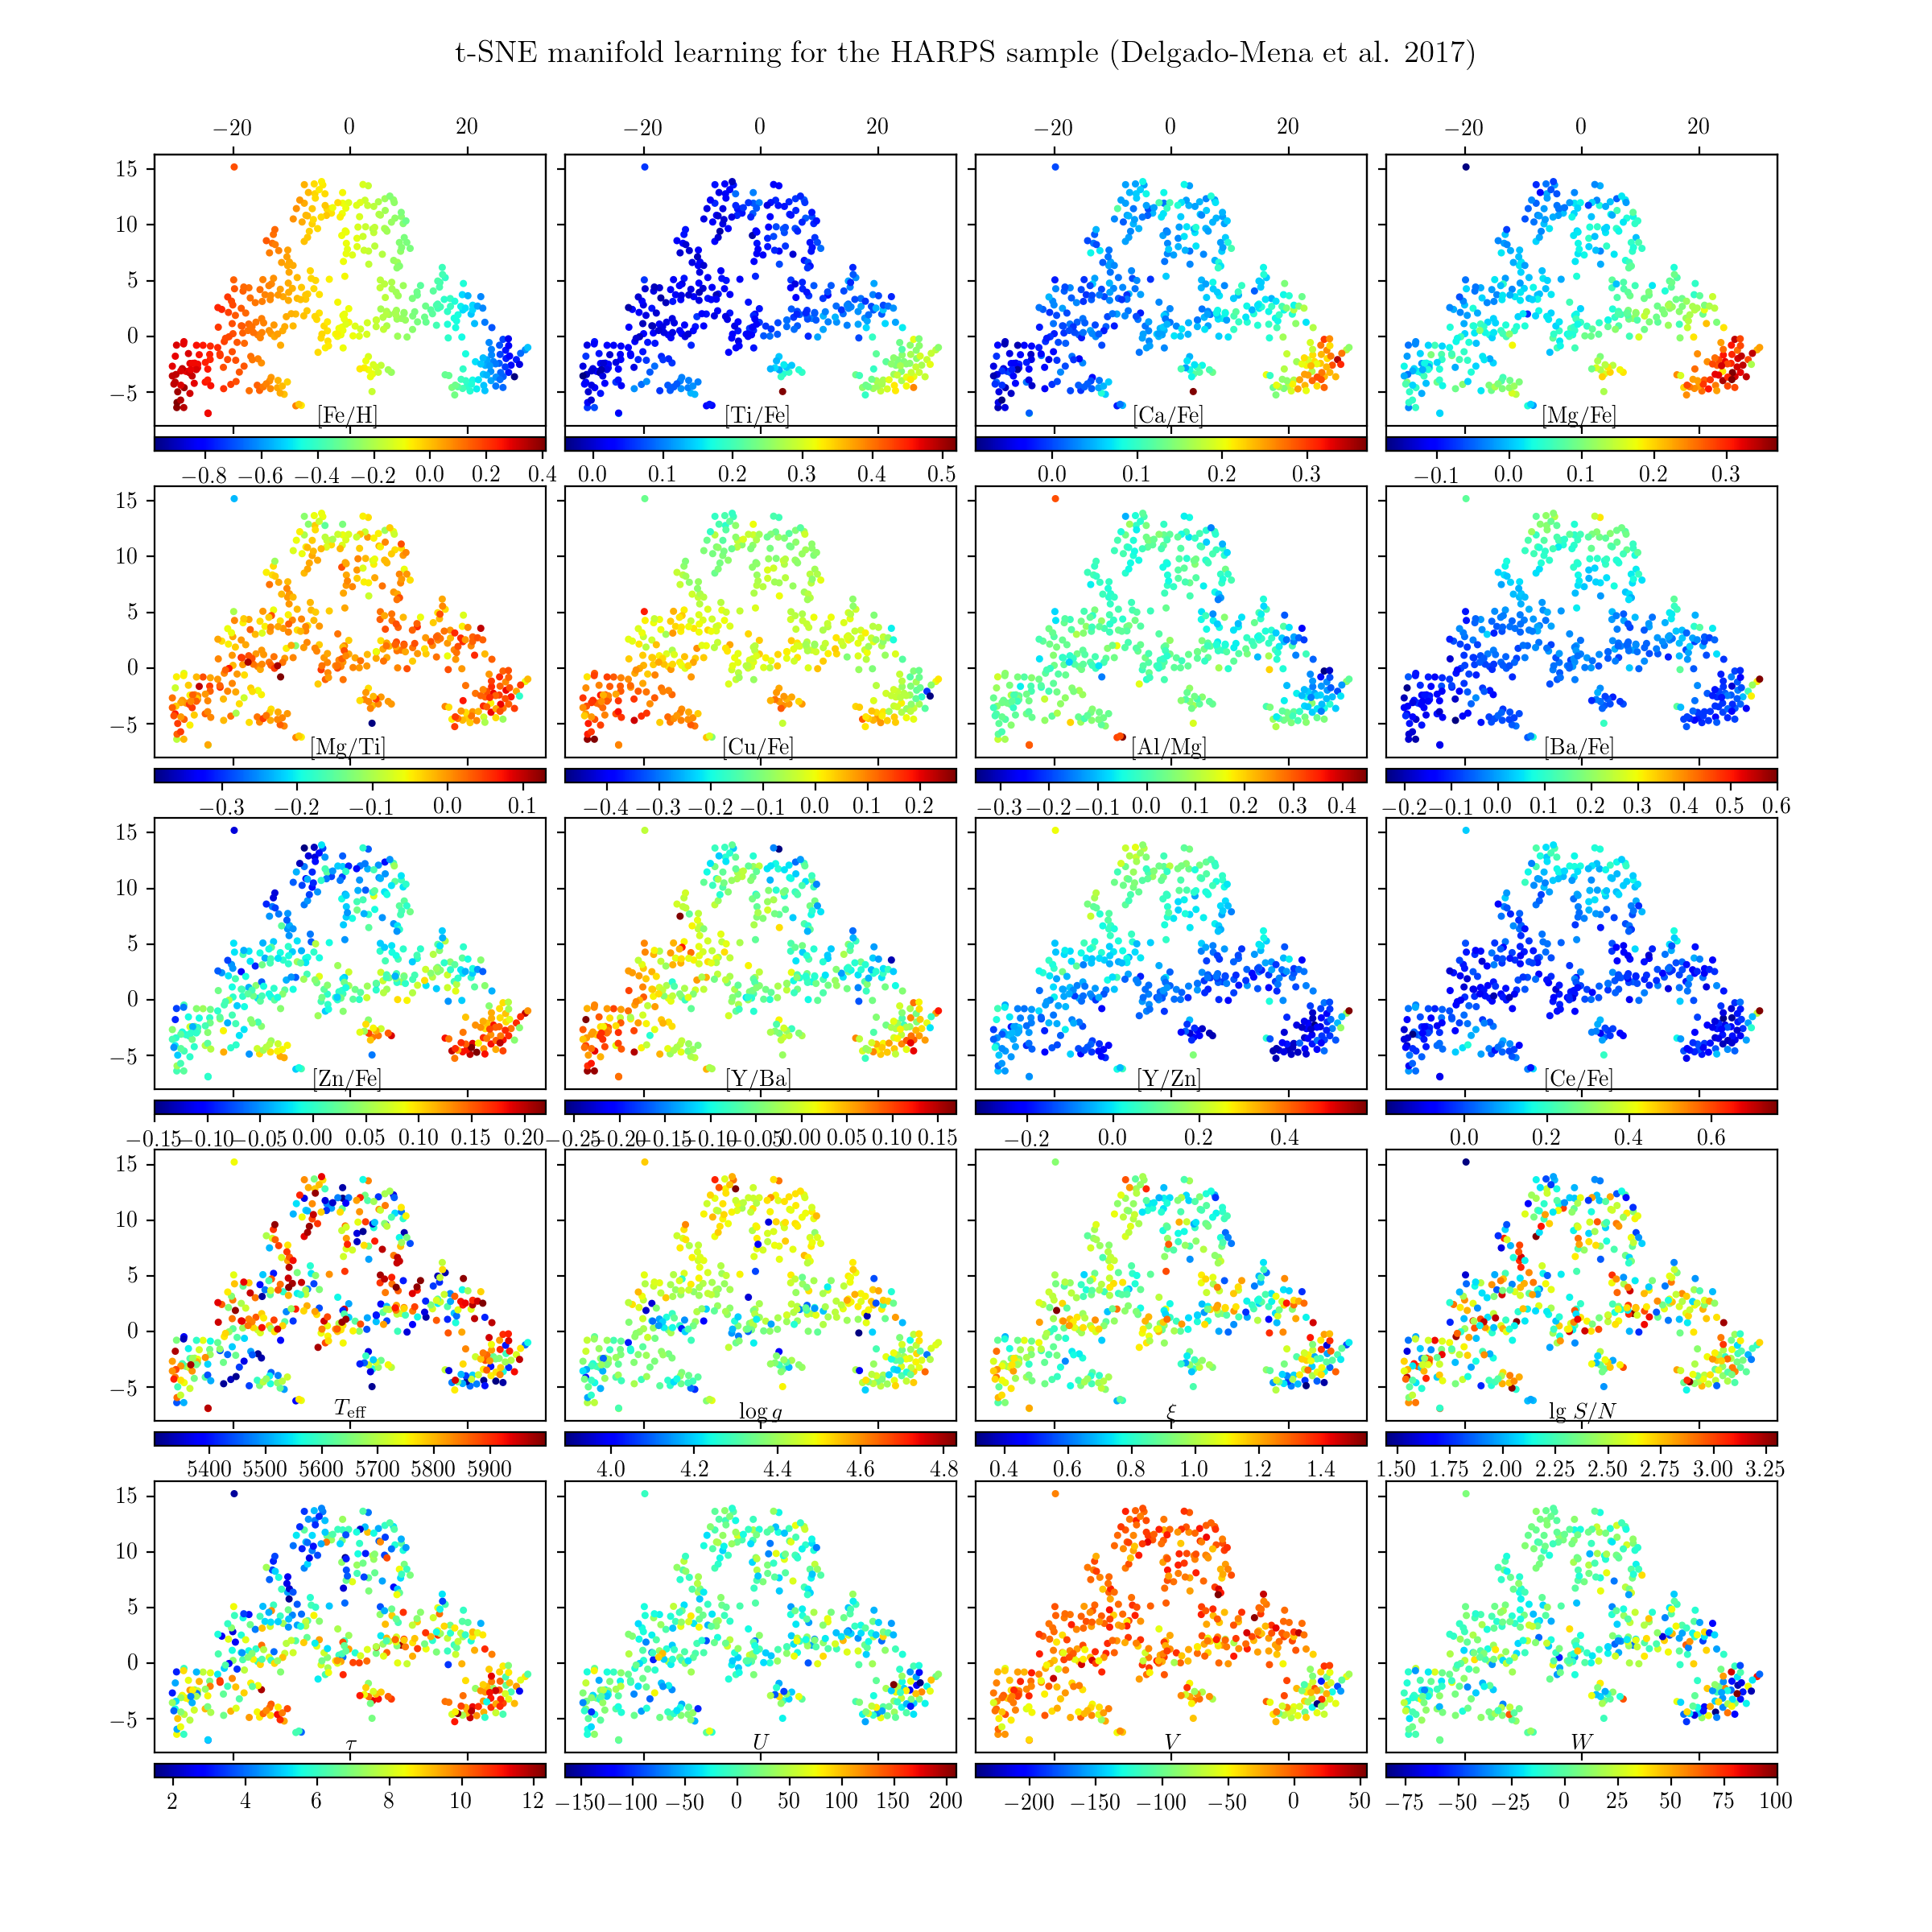
\includegraphics[width=0.99\textwidth]{im/HARPS_tsne_plots_withteffcut40_rand0.png}
\caption{Fiducial t-SNE projection ($p=40$) of the \citet{DelgadoMena2017} sample, colour-coded by chemical abundances (top three rows), stellar atmospheric parameters and signal-to-noise ratio (fourth row), age (fifth row, first panel) and UVW velocities (fifth row). We note that only [Fe/H] and the [X/Fe] ratios were used as input for the t-SNE run. The distinct populations appearing in these diagrams are studied in detail in Fig. \ref{harps2}.}
\label{harps1}
\end{figure*}

In an extensive series of papers, \citet{Adibekyan2011, Adibekyan2012, DelgadoMena2014, DelgadoMena2015, BertrandeLis2015, Suarez-Andres2017, DelgadoMena2017, DelgadoMena2017a} studied the chemical abundances of a sample of 1111 solar-vicinity FGK stars using the very high resolution of the HARPS spectrograph ($R\sim 115,000$). This sample mostly contains metal-rich warm dwarf and subgiant stars, but also includes a wide range of effective temperatures, gravities and metallicities. The HARPS sample initially served to detect and characterise exoplanets and may therefore contain some metallicity-related selection bias; however, e.g. \citet{Anders2014} have shown that the HARPS metallicity distribution (MDF) matches the MDF of high-quality local ($d<1$ kpc) APOGEE red-giant stars that could be considered less chemically biased. 

\citet{DelgadoMena2017} recently reanalysed this sample, employing a revised linelist \citep{Tsantaki2013}, improving the effective temperature calibration, and correcting spectroscopic gravities using the {\it Hipparcos} parallaxes of \citet{vanLeeuwen2007}. They report chemical abundances for Mg, Al, Si, Ca, Ti, Fe, Cu, Zn, Sr, Y, Zr and Ba for 1059 stars (Ce, Nd and Eu are available for a substantial subset of these), derived using standard Local Thermodynamic Equilibrium (LTE) analysis using ARES to measure equivalent widths and MOOG to measure abundances by comparing to Kurucz ATLAS9 atmospheres. In this section we test the performance of abundance-space t-SNE on this most recent HARPS GTO sample compilation. The high number of measured abundances, in conjunction with the high precision of the measurements and the reasonable sample size, makes the HARPS sample an ideal test case for our machine-learning algorithm.  

Our first tests showed that, in order to obtain reliable t-SNE abundance maps, the sample needed to be analysed in a more restricted temperature range, because certain abundance trends seem to be dominated by underlying temperature trends. Therefore, similar to \citet{DelgadoMena2017}, we chose an effective temperature range of 5300 K $<T_{\rm eff}<$ 6000 K for our analysis. We furthermore restricted surface gravities to $3<\log g_{\rm HIP}<5$, and required successful abundance determination for Mg, Al, Si, Ca, TiI, Fe, Cu, Zn, Sr, Y, ZrII, Ce and Ba that we use as input for t-SNE, leaving us with 533 stars.\footnote{Carbon and oxygen estimates are available from previous studies \citep{Suarez-Andres2017, BertrandeLis2015}, but since they are based on previous stellar parameter estimates, we decided to only use them in the interpretation. We also did not use Nd and Eu in the t-SNE run, because they were only available for about half of the sample (stars with the highest signal-to-noise ratios). We do, however, use the Nd and Eu results in the interpretation, whenever they are available.} In our final sample of 530 stars we also discarded 3 stars for which our age determination code, {\tt StarHorse} \citep{Santiago2016, Queiroz2017}, did not converge. We verified that these choices do not significantly affect the resulting t-SNE maps. 

The chemical abundances were complemented by astrometric data (parallaxes, proper motions) from the Gaia/TGAS catalogue \citet{GaiaCollaboration2016}, or when these were unavailable (135/1059 stars), from the re-reduced {\it Hipparcos} data \citep{vanLeeuwen2007}. {\bf DESCRIBE StarHorse RUN HERE}.

Fig. \ref{harps1} again shows our reference t-SNE map for the HARPS sample, but now colour-coded by chemical-abundance ratios, stellar parameters, ages and kinematics. The panels in the first three rows show how t-SNE is grouping the stars with similar abundances in the two-dimensional plane. The panels coloured as a function of stellar parameters demonstrate that the sample is not subject to major systematic abundance shifts, but does show some residual trends with effective temperature, since it preferentially groups cooler stars in slightly different regions of the t-SNE map than hotter ones. Because part of this effect may be due to chemical evolution rather than systematic abundance errors, we decided not to apply any ad-hoc corrections to the abundances. 

We identified some of the substructures that appear in Fig. \ref{harps1} already in Fig. \ref{harps0}. Fig. \ref{harps3} shows the corresponding [X/Fe] abundance trends versus proton number for each of those substructures.

We now proceed to the discussion of these results.

\subsection{The overall appearance of the t-SNE map}



\begin{figure}\centering
 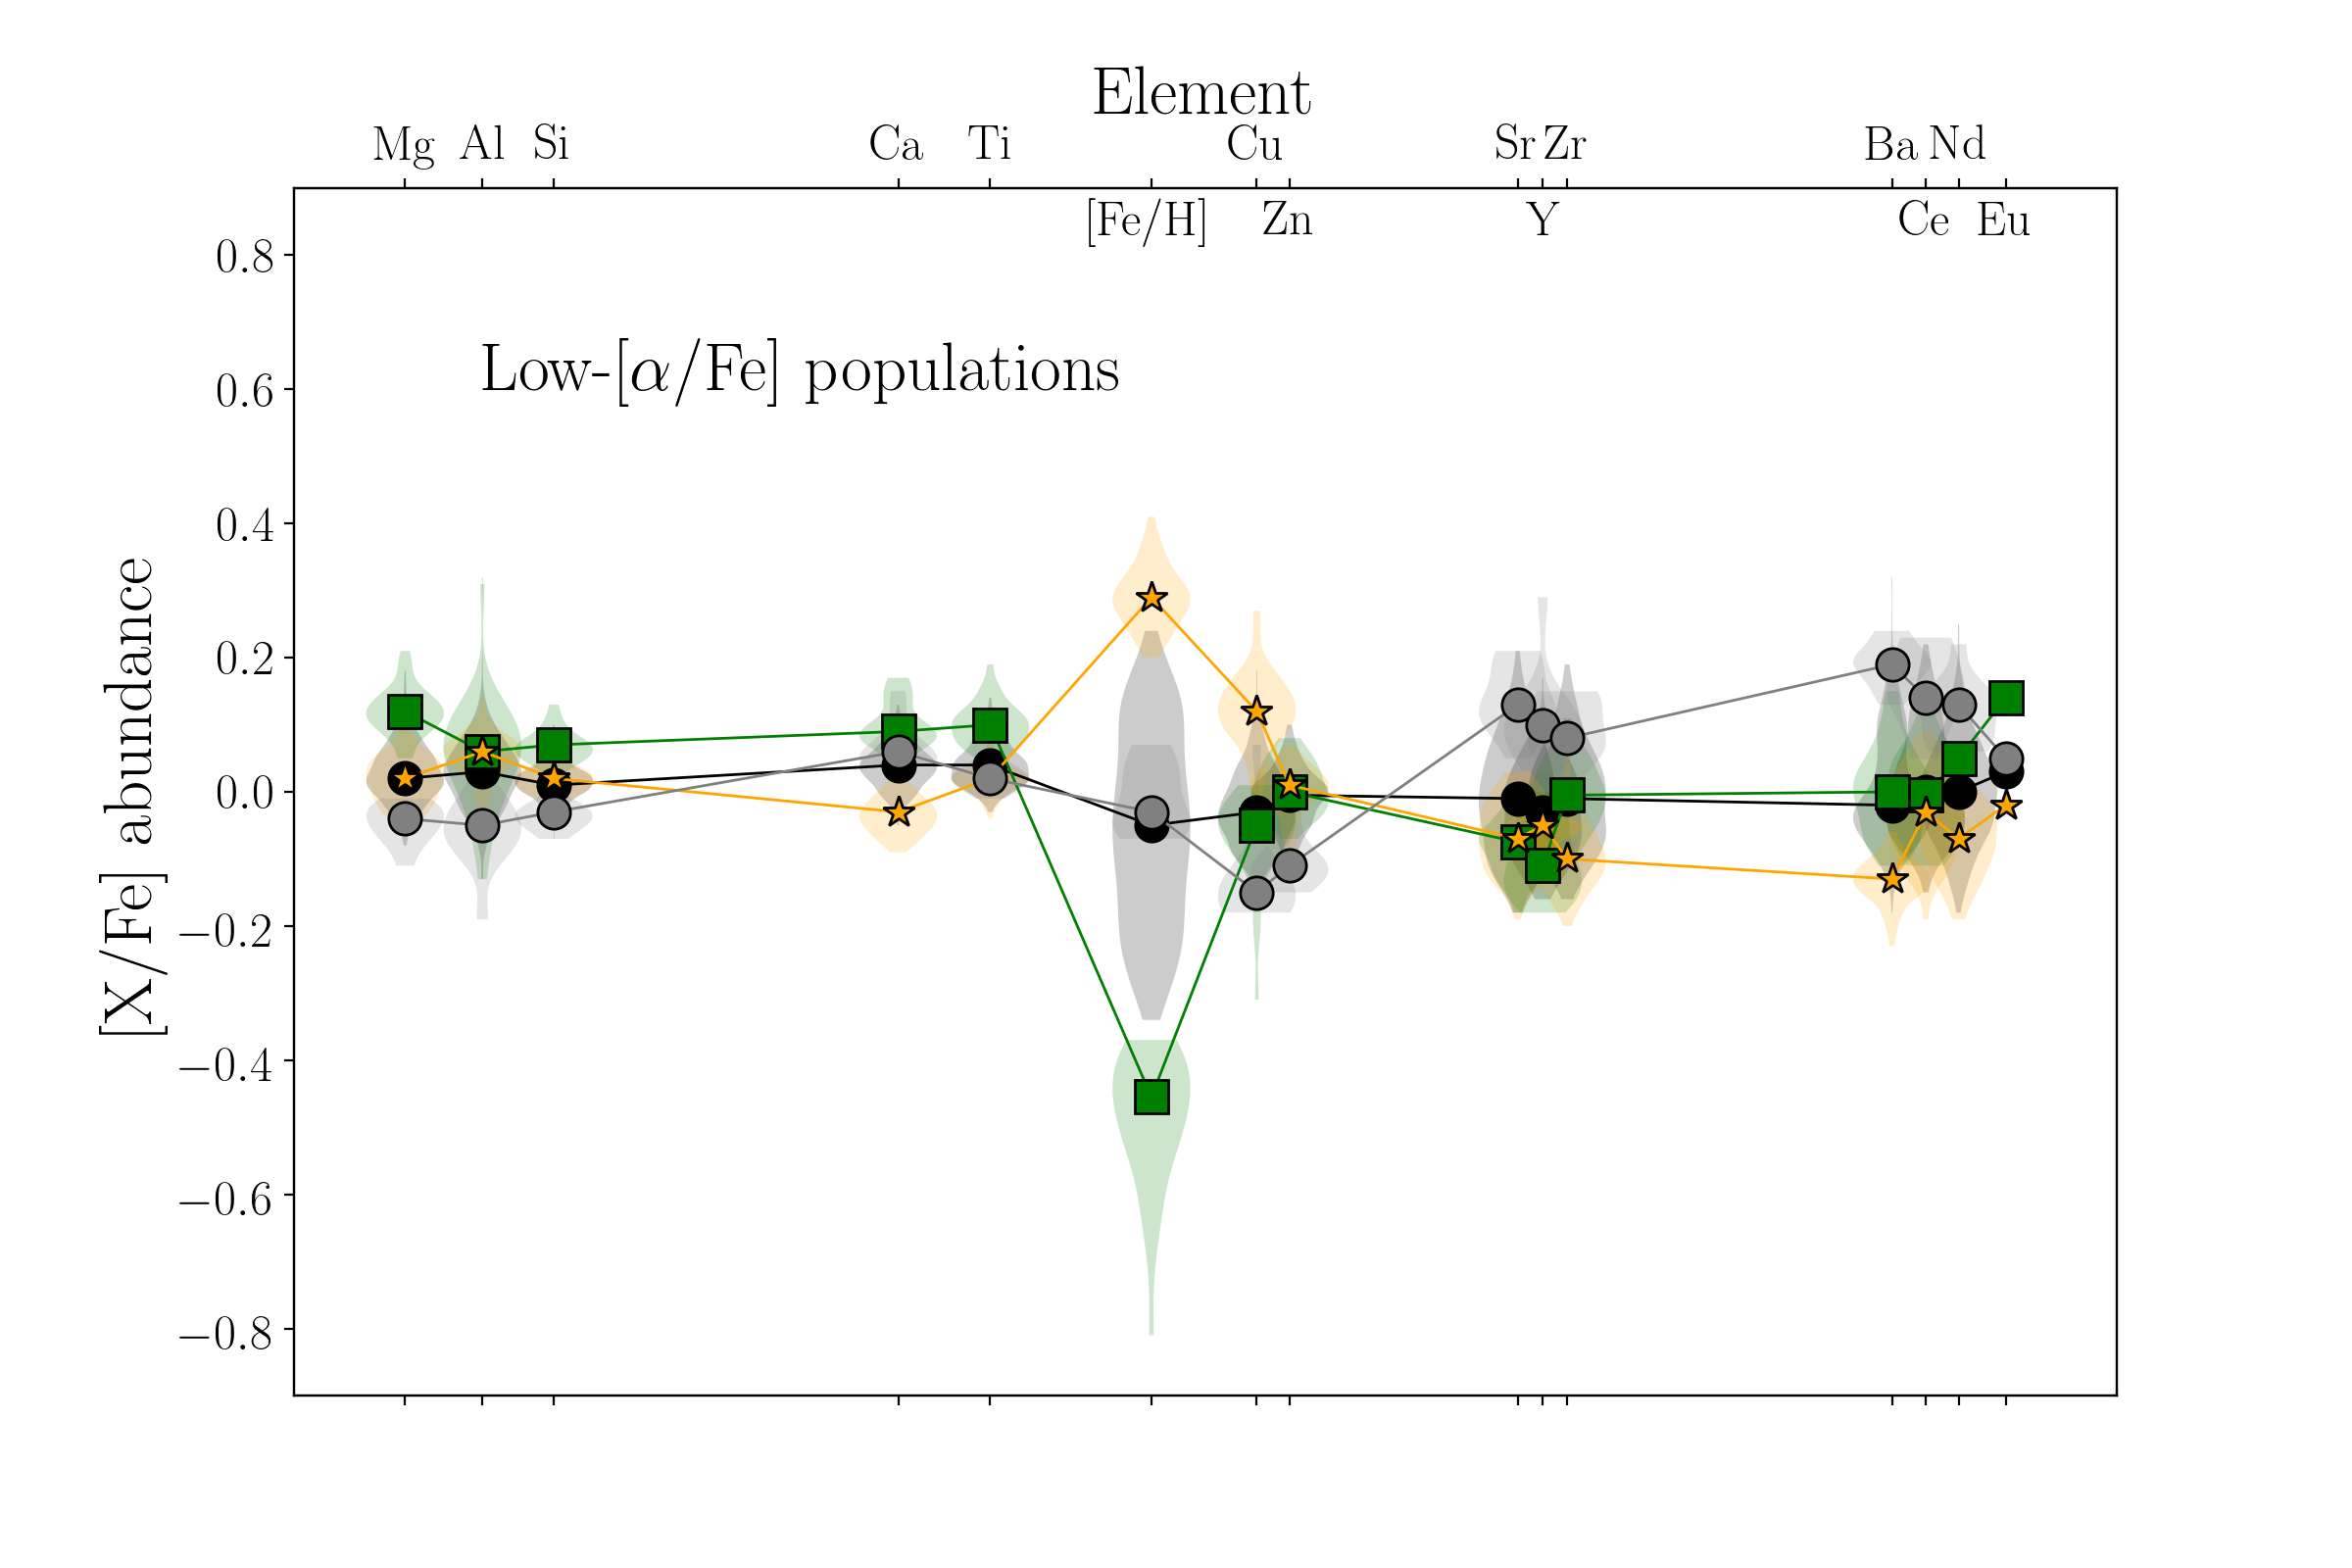
\includegraphics[trim=0cm 2cm 0cm 0cm, clip=true, width=0.49\textwidth]{im/harps_tsne_abundances-relto-Fe_thin.png}
 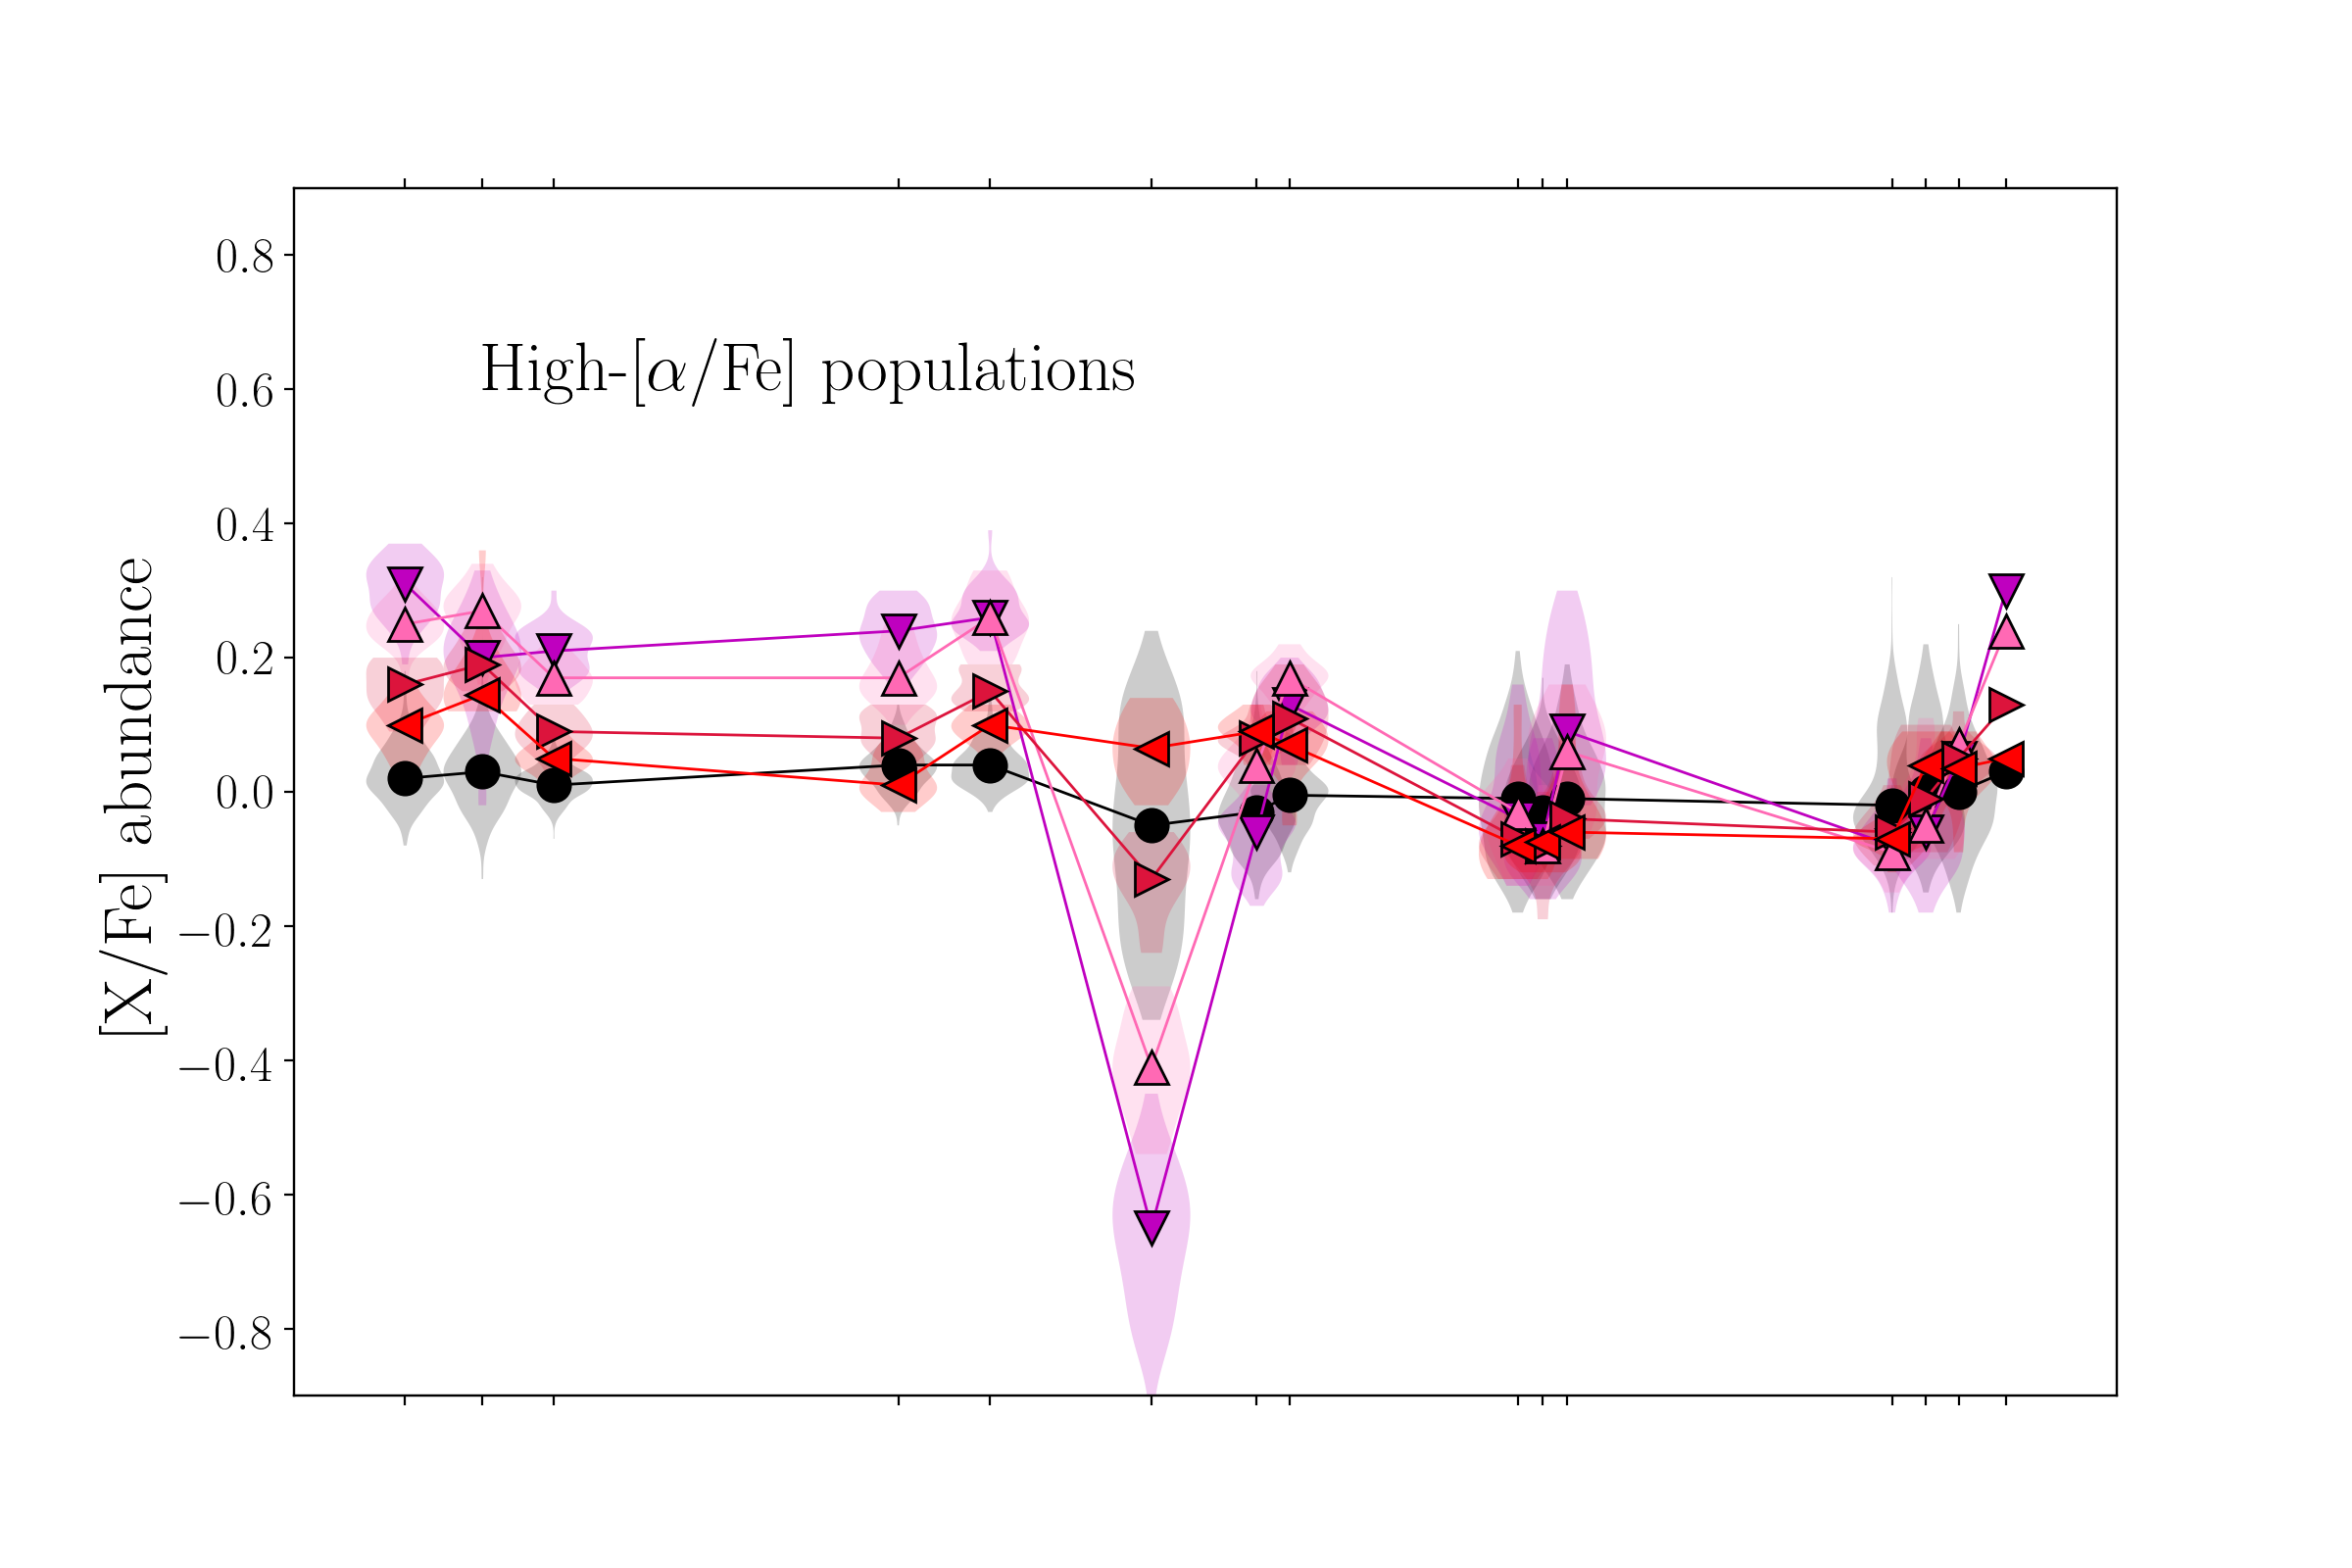
\includegraphics[trim=0cm 2cm 0cm 2cm, clip=true, width=0.49\textwidth]{im/harps_tsne_abundances-relto-Fe_thick.png}
 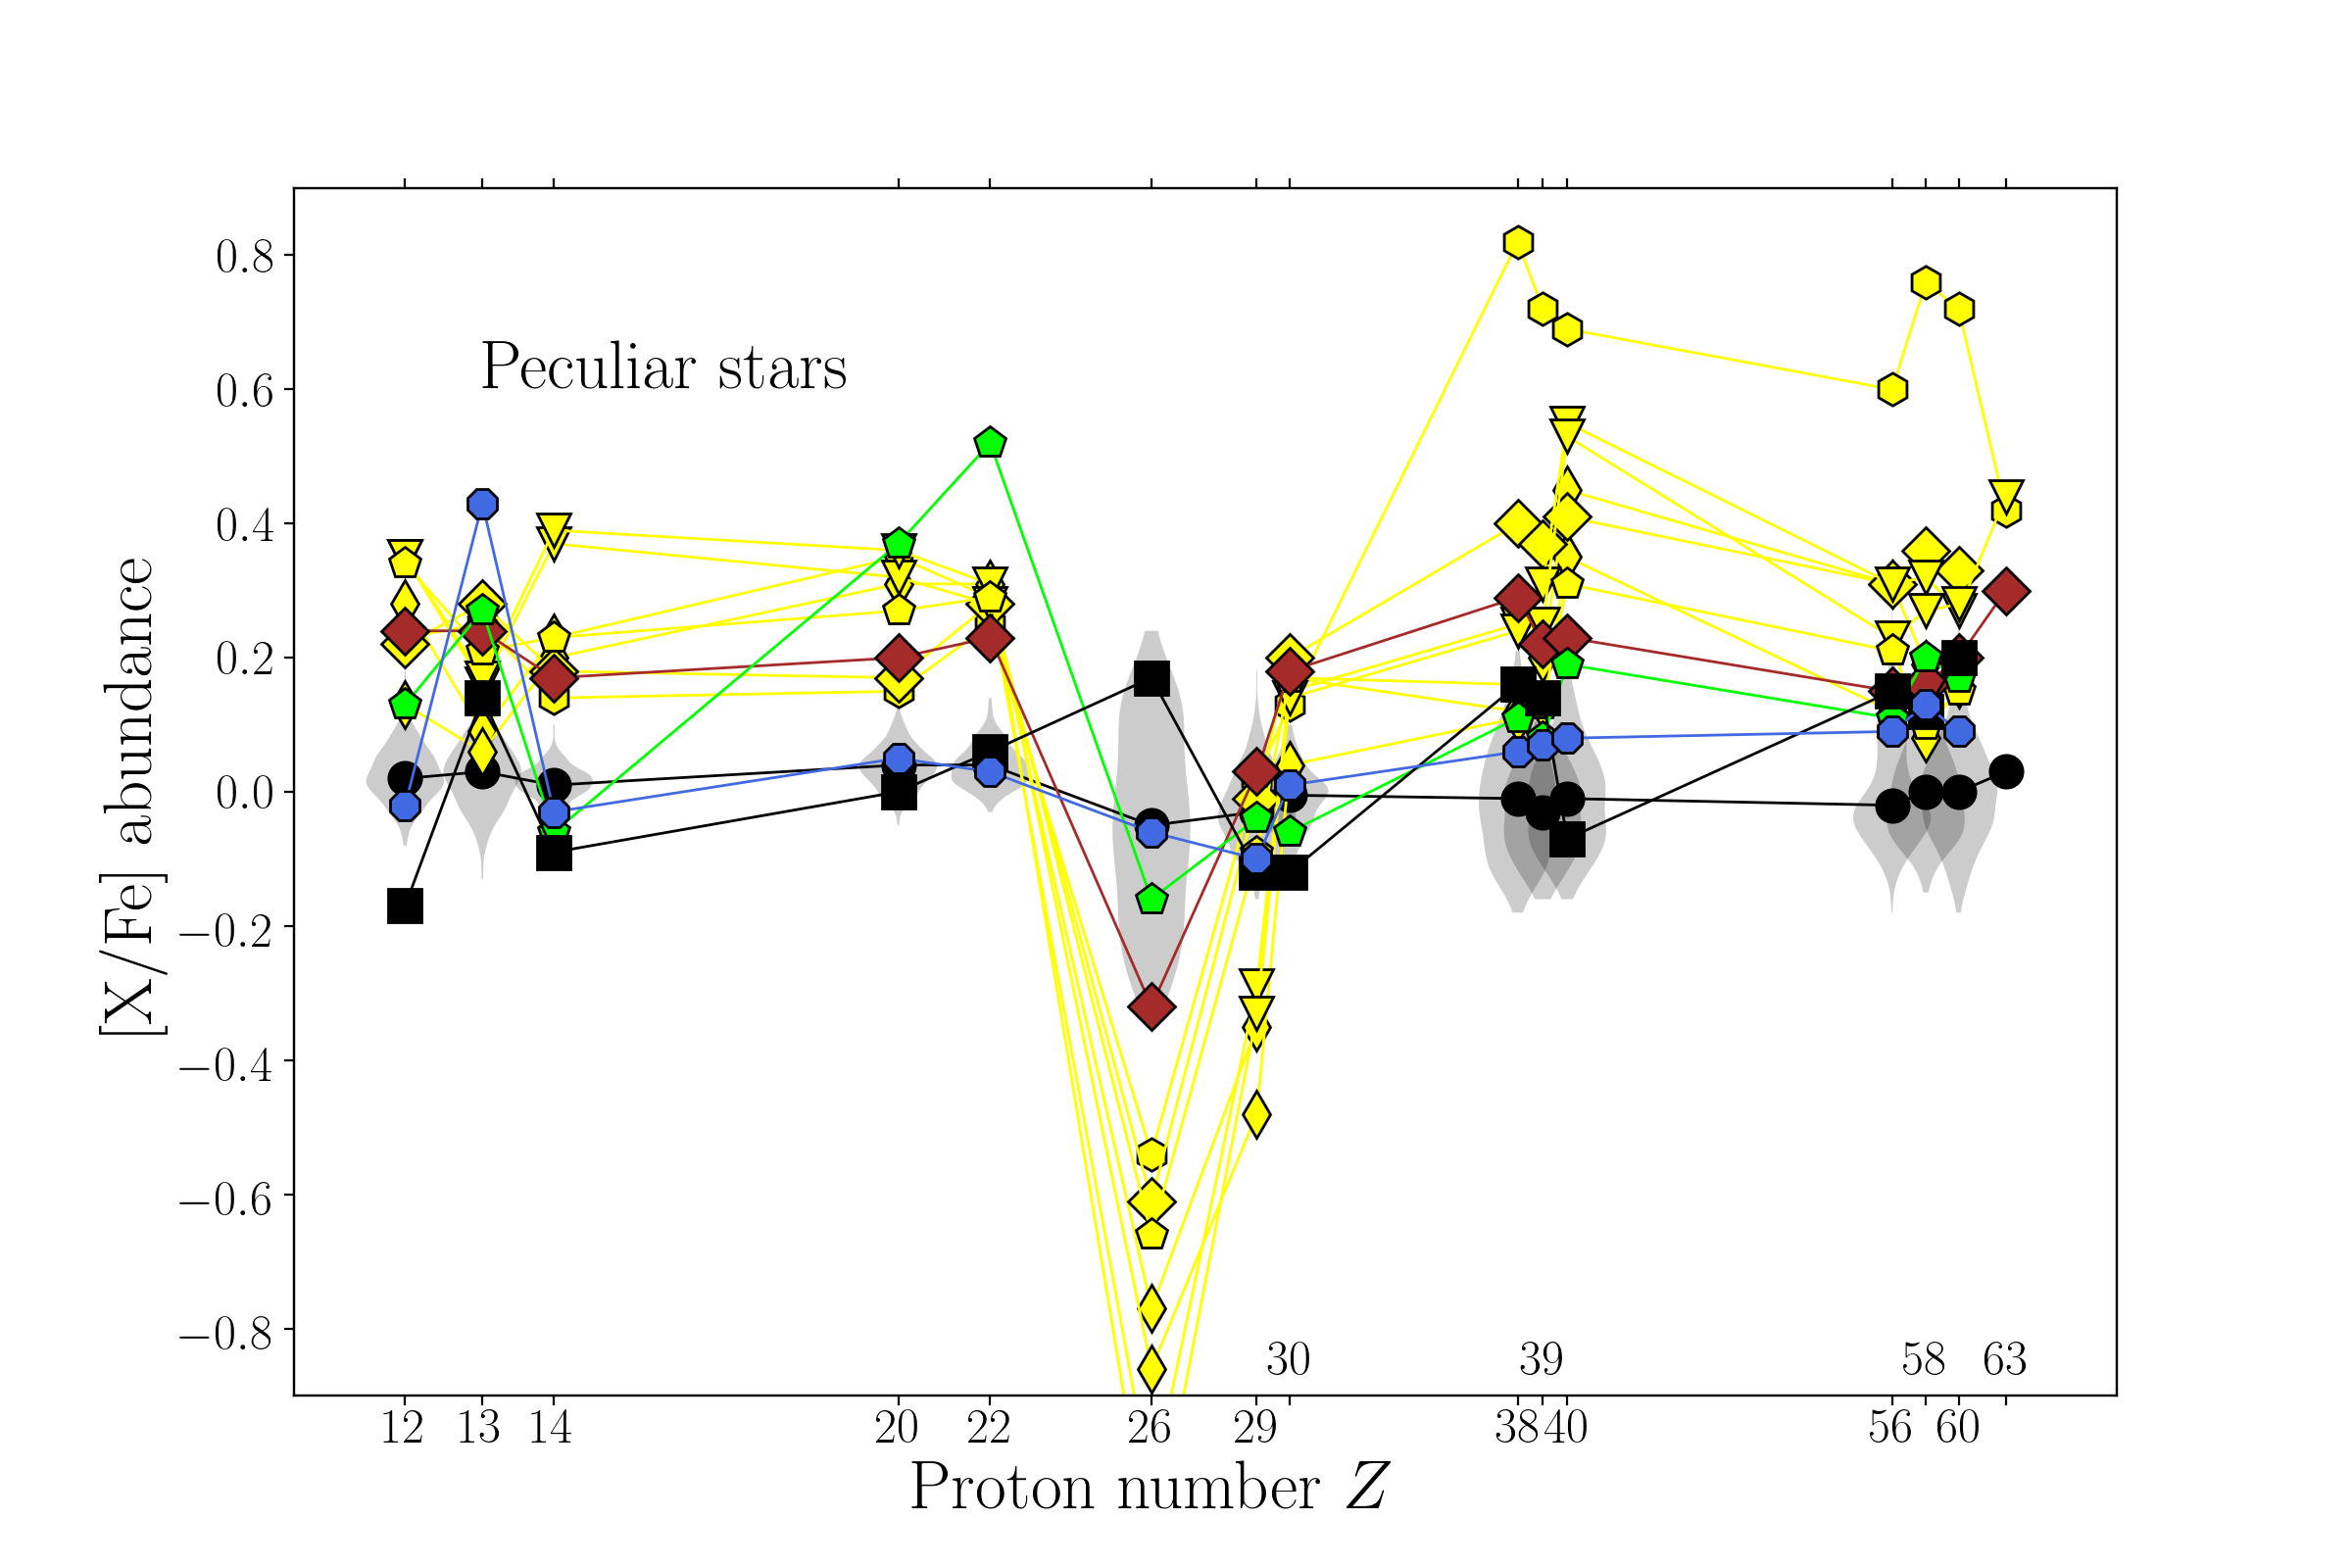
\includegraphics[trim=0cm 0 0cm 2cm, clip=true, width=0.49\textwidth]{im/harps_tsne_abundances-relto-Fe_strange.png}
\caption{Chemical-abundance patterns relative to iron for the t-SNE-selected subsamples of the HARPS survey. For visibility, we show only the median abundance ratios of each group.}
\label{harps3}
\end{figure}

\subsection{The robustness of the t-SNE results}

\begin{figure}\centering
 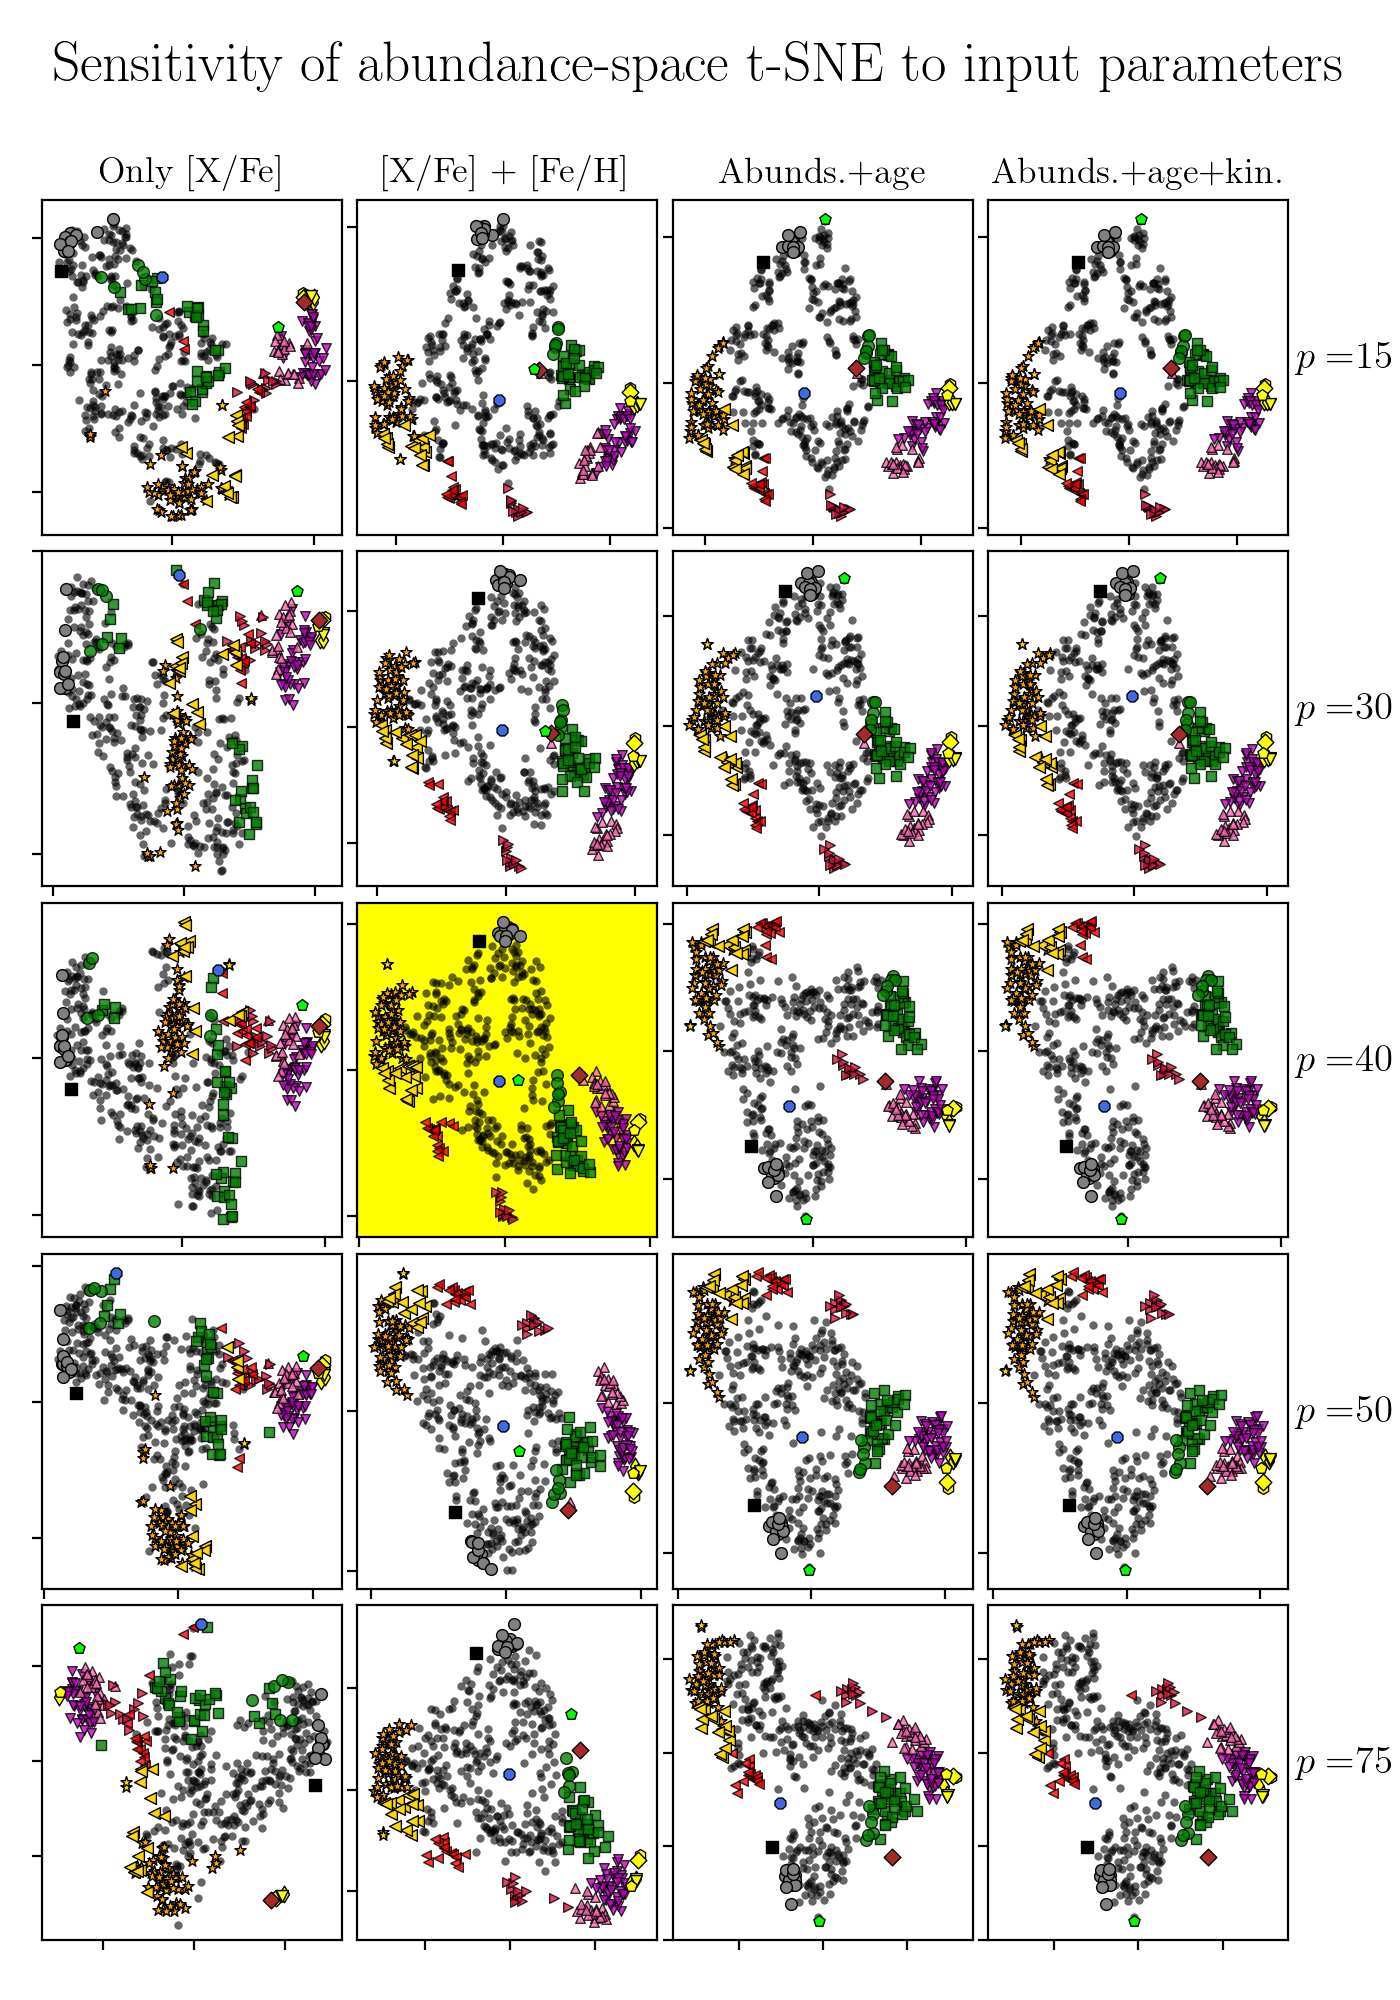
\includegraphics[width=0.49\textwidth]{im/harps-tSNE_perplexitytest_withsubsets.png}
\caption{t-SNE representations of the chrono-chemo-kinematics space spanned by the \citet{DelgadoMena2017} sample. Each column row represents a combination of input information, while each row corresponds to a particular perplexity value, as indicated on the right side of the figure. The panel highlighted in yellow represents the results that we analyse in detail in this paper by defining chemical subpopulations based on this map.}
\label{perplexitytest2}
\end{figure}

\begin{figure}\centering
 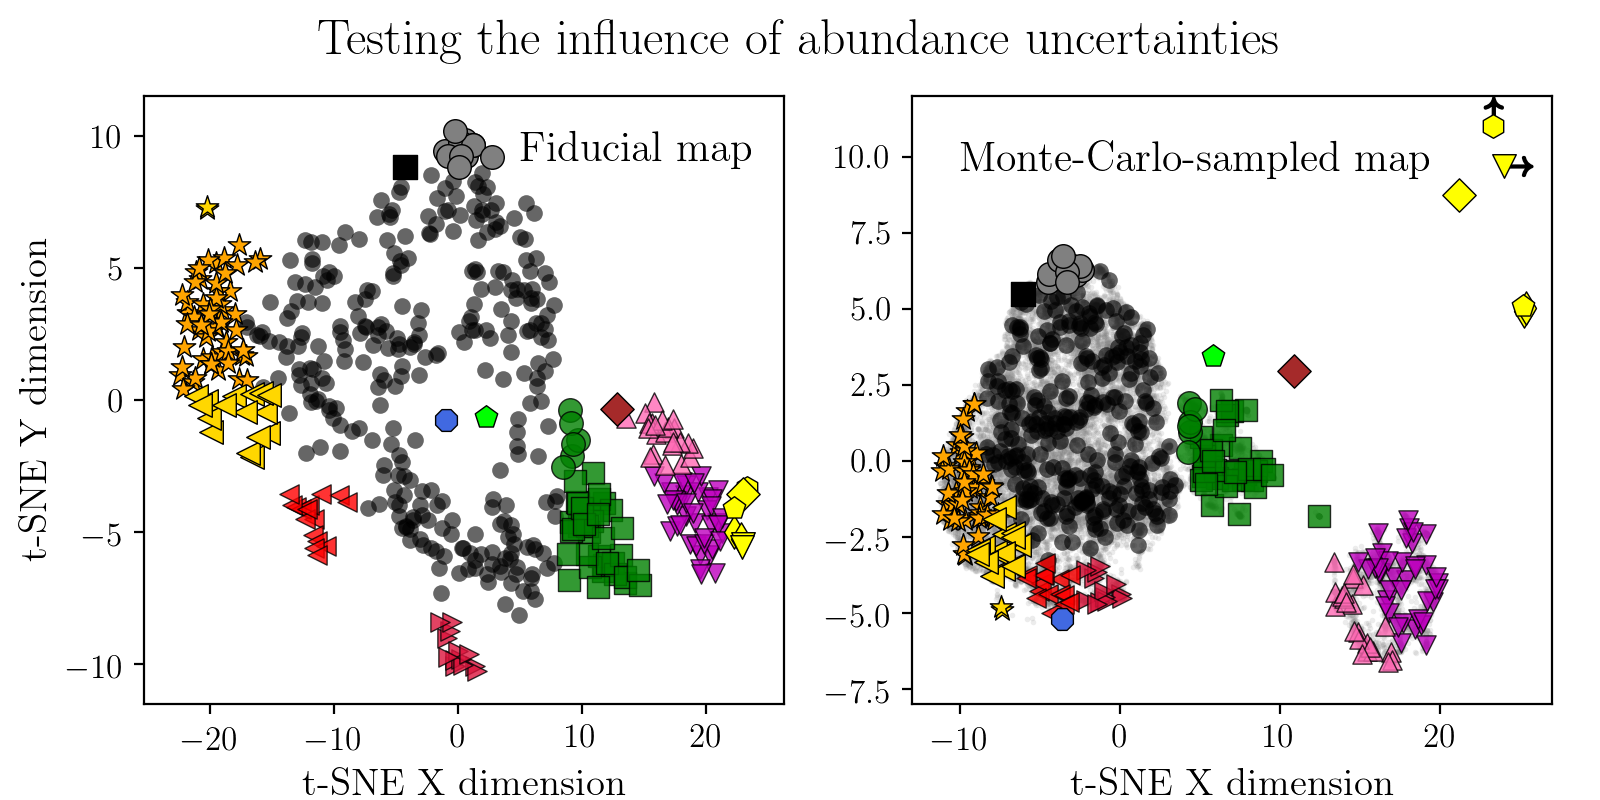
\includegraphics[width=0.49\textwidth]{im/harps_tsne-mctest_teffcut.png}
\caption{Robustness test of our t-SNE-selected subsamples. The right panel shows the fiducial map, while the left panel shows the result of our Monte-Carlo test. For each star, 50 random stars were drawn from the a Gaussian centered on the measured abundance, and with widths corresponding to the measured uncertainties. The resulting map demonstrates that our selected subgroups are robust to measurement errors.}
\label{harps2}
\end{figure}

We tested the robustness of our reference map with a simple Monte-Carlo experiment: For each star, we created 50 mock stars with abundances drawn from a multi-dimensional Gaussian distribution centered on the measured abundance, and variance corresponding to the measured abundance uncertainties. Although t-SNE does not take into account uncertainties in the data, this procedure allows us to assure that the groups that we identified in the t-SNE map are not due to chance groupings.\footnote{In general, adding uncertainties to measured (i.e. already noisy) data will blur the true values even more. This means that if a signal disappears in the Monte-Carlo test, the test does not rule out the existence of the signal. On the other hand, if the signal persists, the signal is very unlikely to be due to a chance grouping.} 

\subsection{The thin-thick disc dichotomy} 

As discussed in the works of \citet{Adibekyan2011, Adibekyan2012} or \citet{DelgadoMena2017}, there is a clear discontinuity between the high- and the low-[$\alpha$/Fe] sequences in the [Mg/Fe] vs. [Fe/H] diagram. This discontinuity is reflected in a very clear manner in the t-SNE projection:
We find a clear and obvious gap between the chemical thin- and thick-disc populations in the t-SNE diagram that remains very robust for different choices of the t-SNE hyper-parameters. Primarily, this means that the chemical patterns of thin and thick disc are indeed distinct, and can be disentangled by high-resolution spectroscopy. Secondly, our analysis of the full chemical information results in a much more accurate division of the chemically-thin and thick populations. Indeed, if one only relies on one diagnostic, such as the [Mg/Fe] vs. [Fe/H] diagram \citep{Adibekyan2011, DelgadoMena2017}, several thin-disc stars would (most probably incorrectly) be identified as belonging chemical thick disc (see Fig. \ref{harps0}). 

\subsection{Sub-populations and chemically peculiar stars}

{\it Thick-disc sub-populations:} \citet{Adibekyan2011} first discovered a clear discontinuity between the metal-poor and metal-rich $[\alpha$/Fe]-enhanced (or h$\alpha$mr) disc populations. In our t-SNE analysis of the \citet{Bensby2014} sample, similar to the original paper, we only see a hint of a difference between the two populations (dubbed Thick Disc I and II in Fig. \ref{bensby1}). The bimodality is better seen when slightly higher perplexity values are chosen ($p\sim 30$). Even if ages and/or kinematics are included as additional dimensions in the analysis, this picture does not change much. 

{\it Thin-thick transition stars:} 

{\it Super-metal-rich stars:} 

{\it The metal-poor thin disc:} 

{\it Satellite debris} 

\subsection{Abundance trends with age}

\begin{figure}\centering
 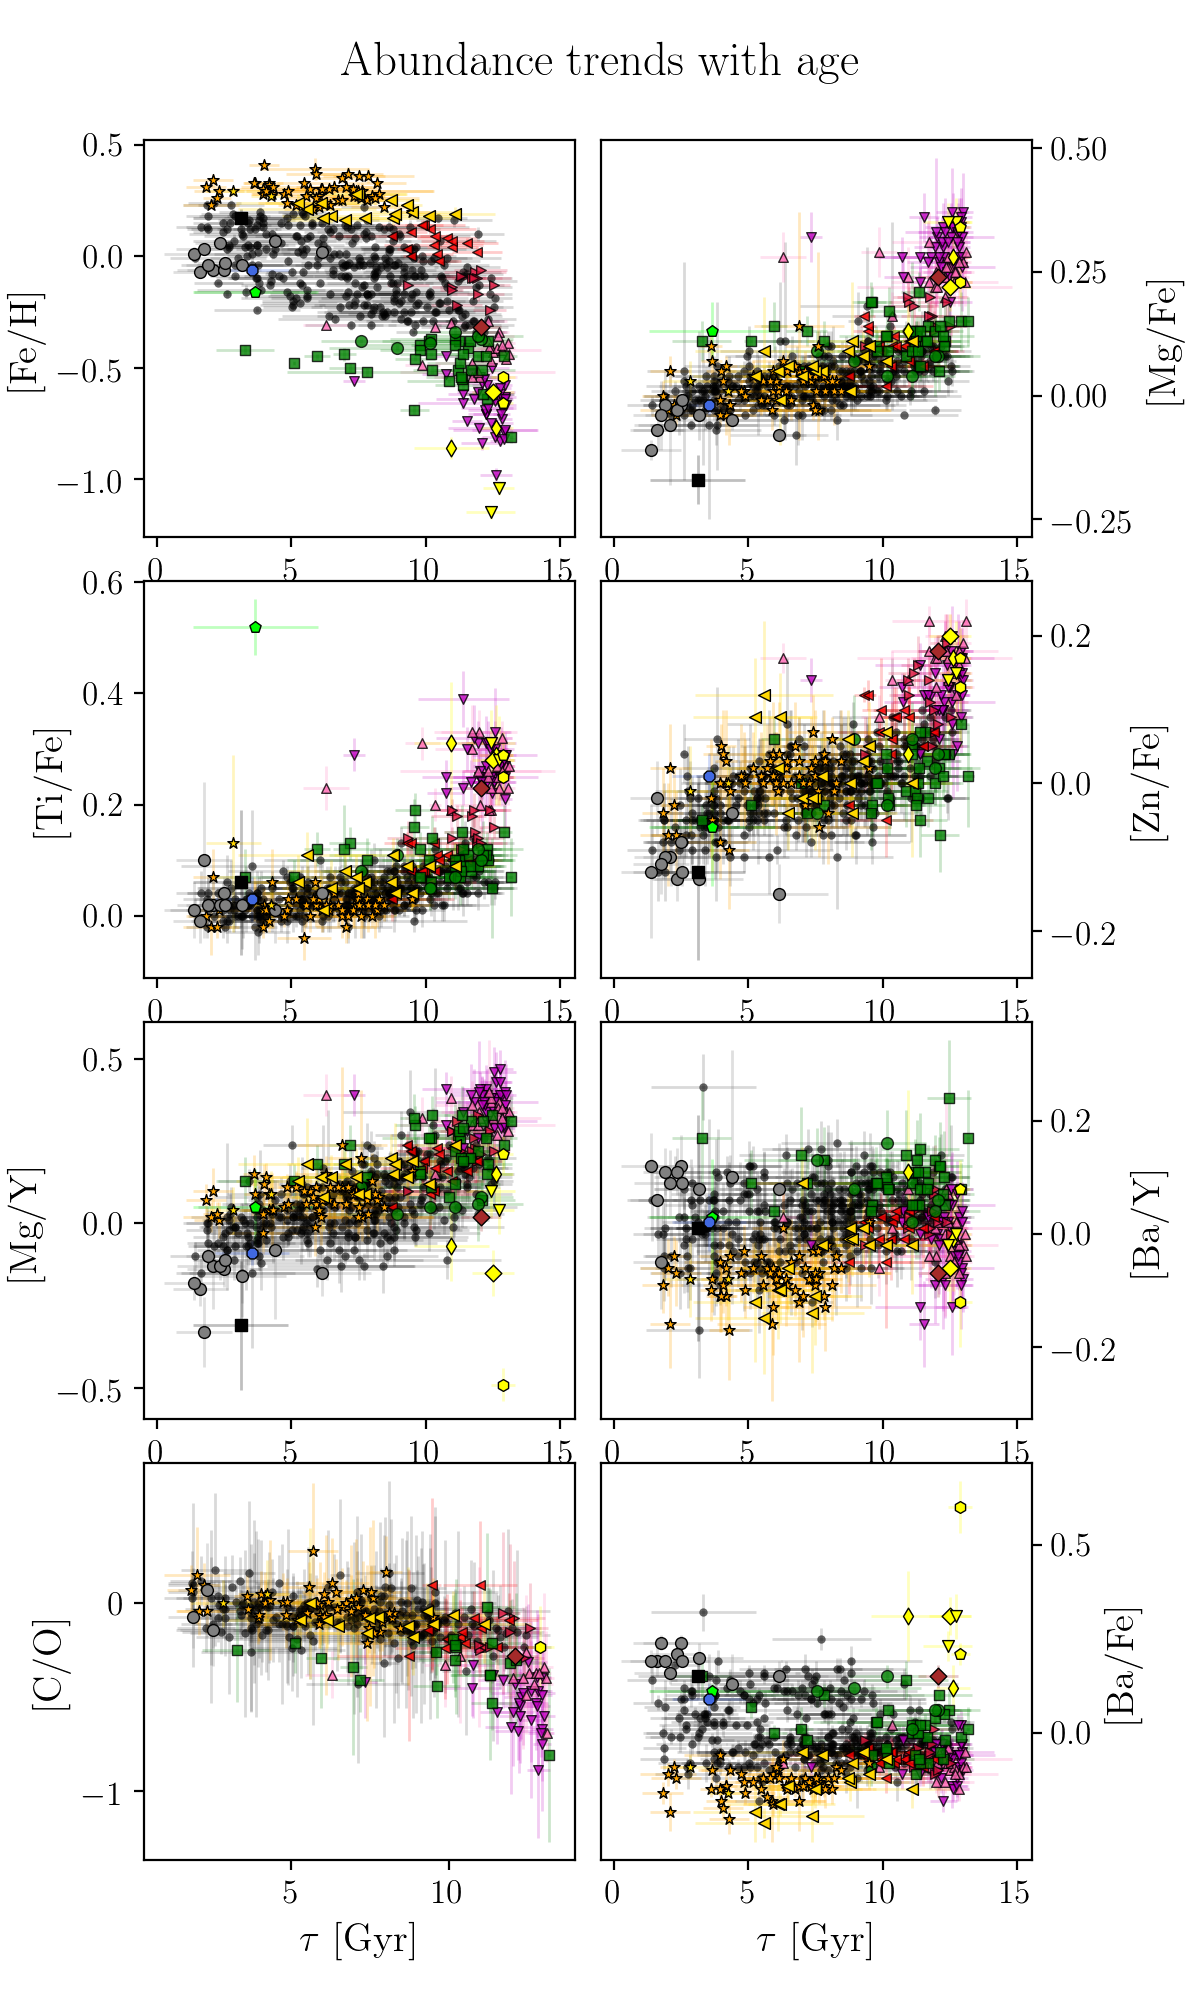
\includegraphics[width=0.49\textwidth]{im/harps_tsne-age-abundsplot_teffcut.png}
\caption{Abundance trends with stellar age, measured with the \texttt{StarHorse} code \citep{Queiroz2017}.}
\label{harps2}
\end{figure}


\subsection{Kinematic trends}

\begin{figure}\centering
 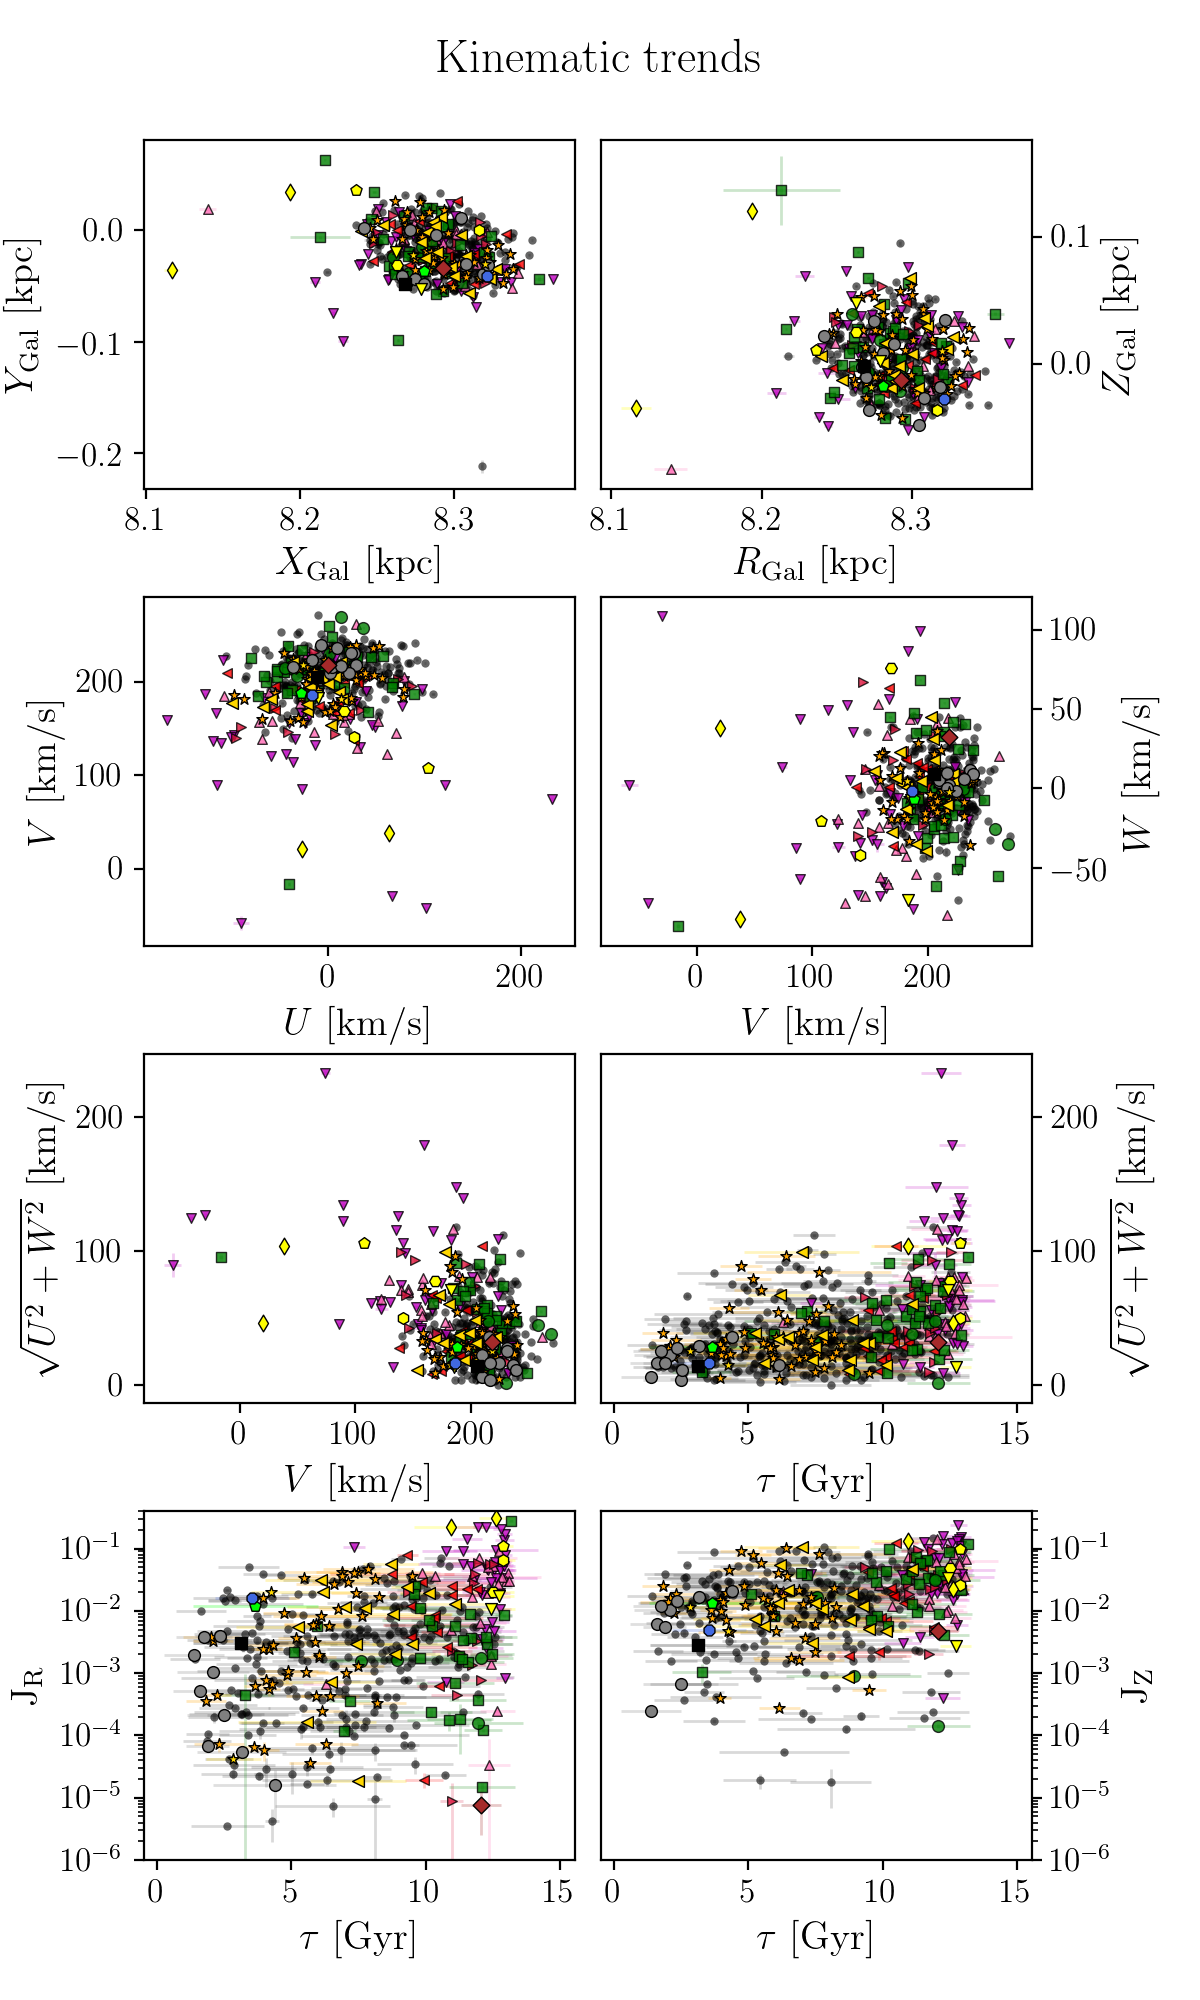
\includegraphics[width=0.49\textwidth]{im/harps_tsne-kin-abundsplot_teffcut.png}
\caption{Abundance trends with stellar age, measured with the \texttt{StarHorse} code \citep{Queiroz2017}.}
\label{harps2}
\end{figure}



% %%%%%%%%%%%%%%%%%%%%%%%%%%%%%%%%%%%%%%%%%%%%%%%
% \section{Re-analysing the \citet{Bensby2014} sample}\label{bensby}
% %%%%%%%%%%%%%%%%%%%%%%%%%%%%%%%%%%%%%%%%%%%%%%%
% 
% \begin{figure*}\centering
%  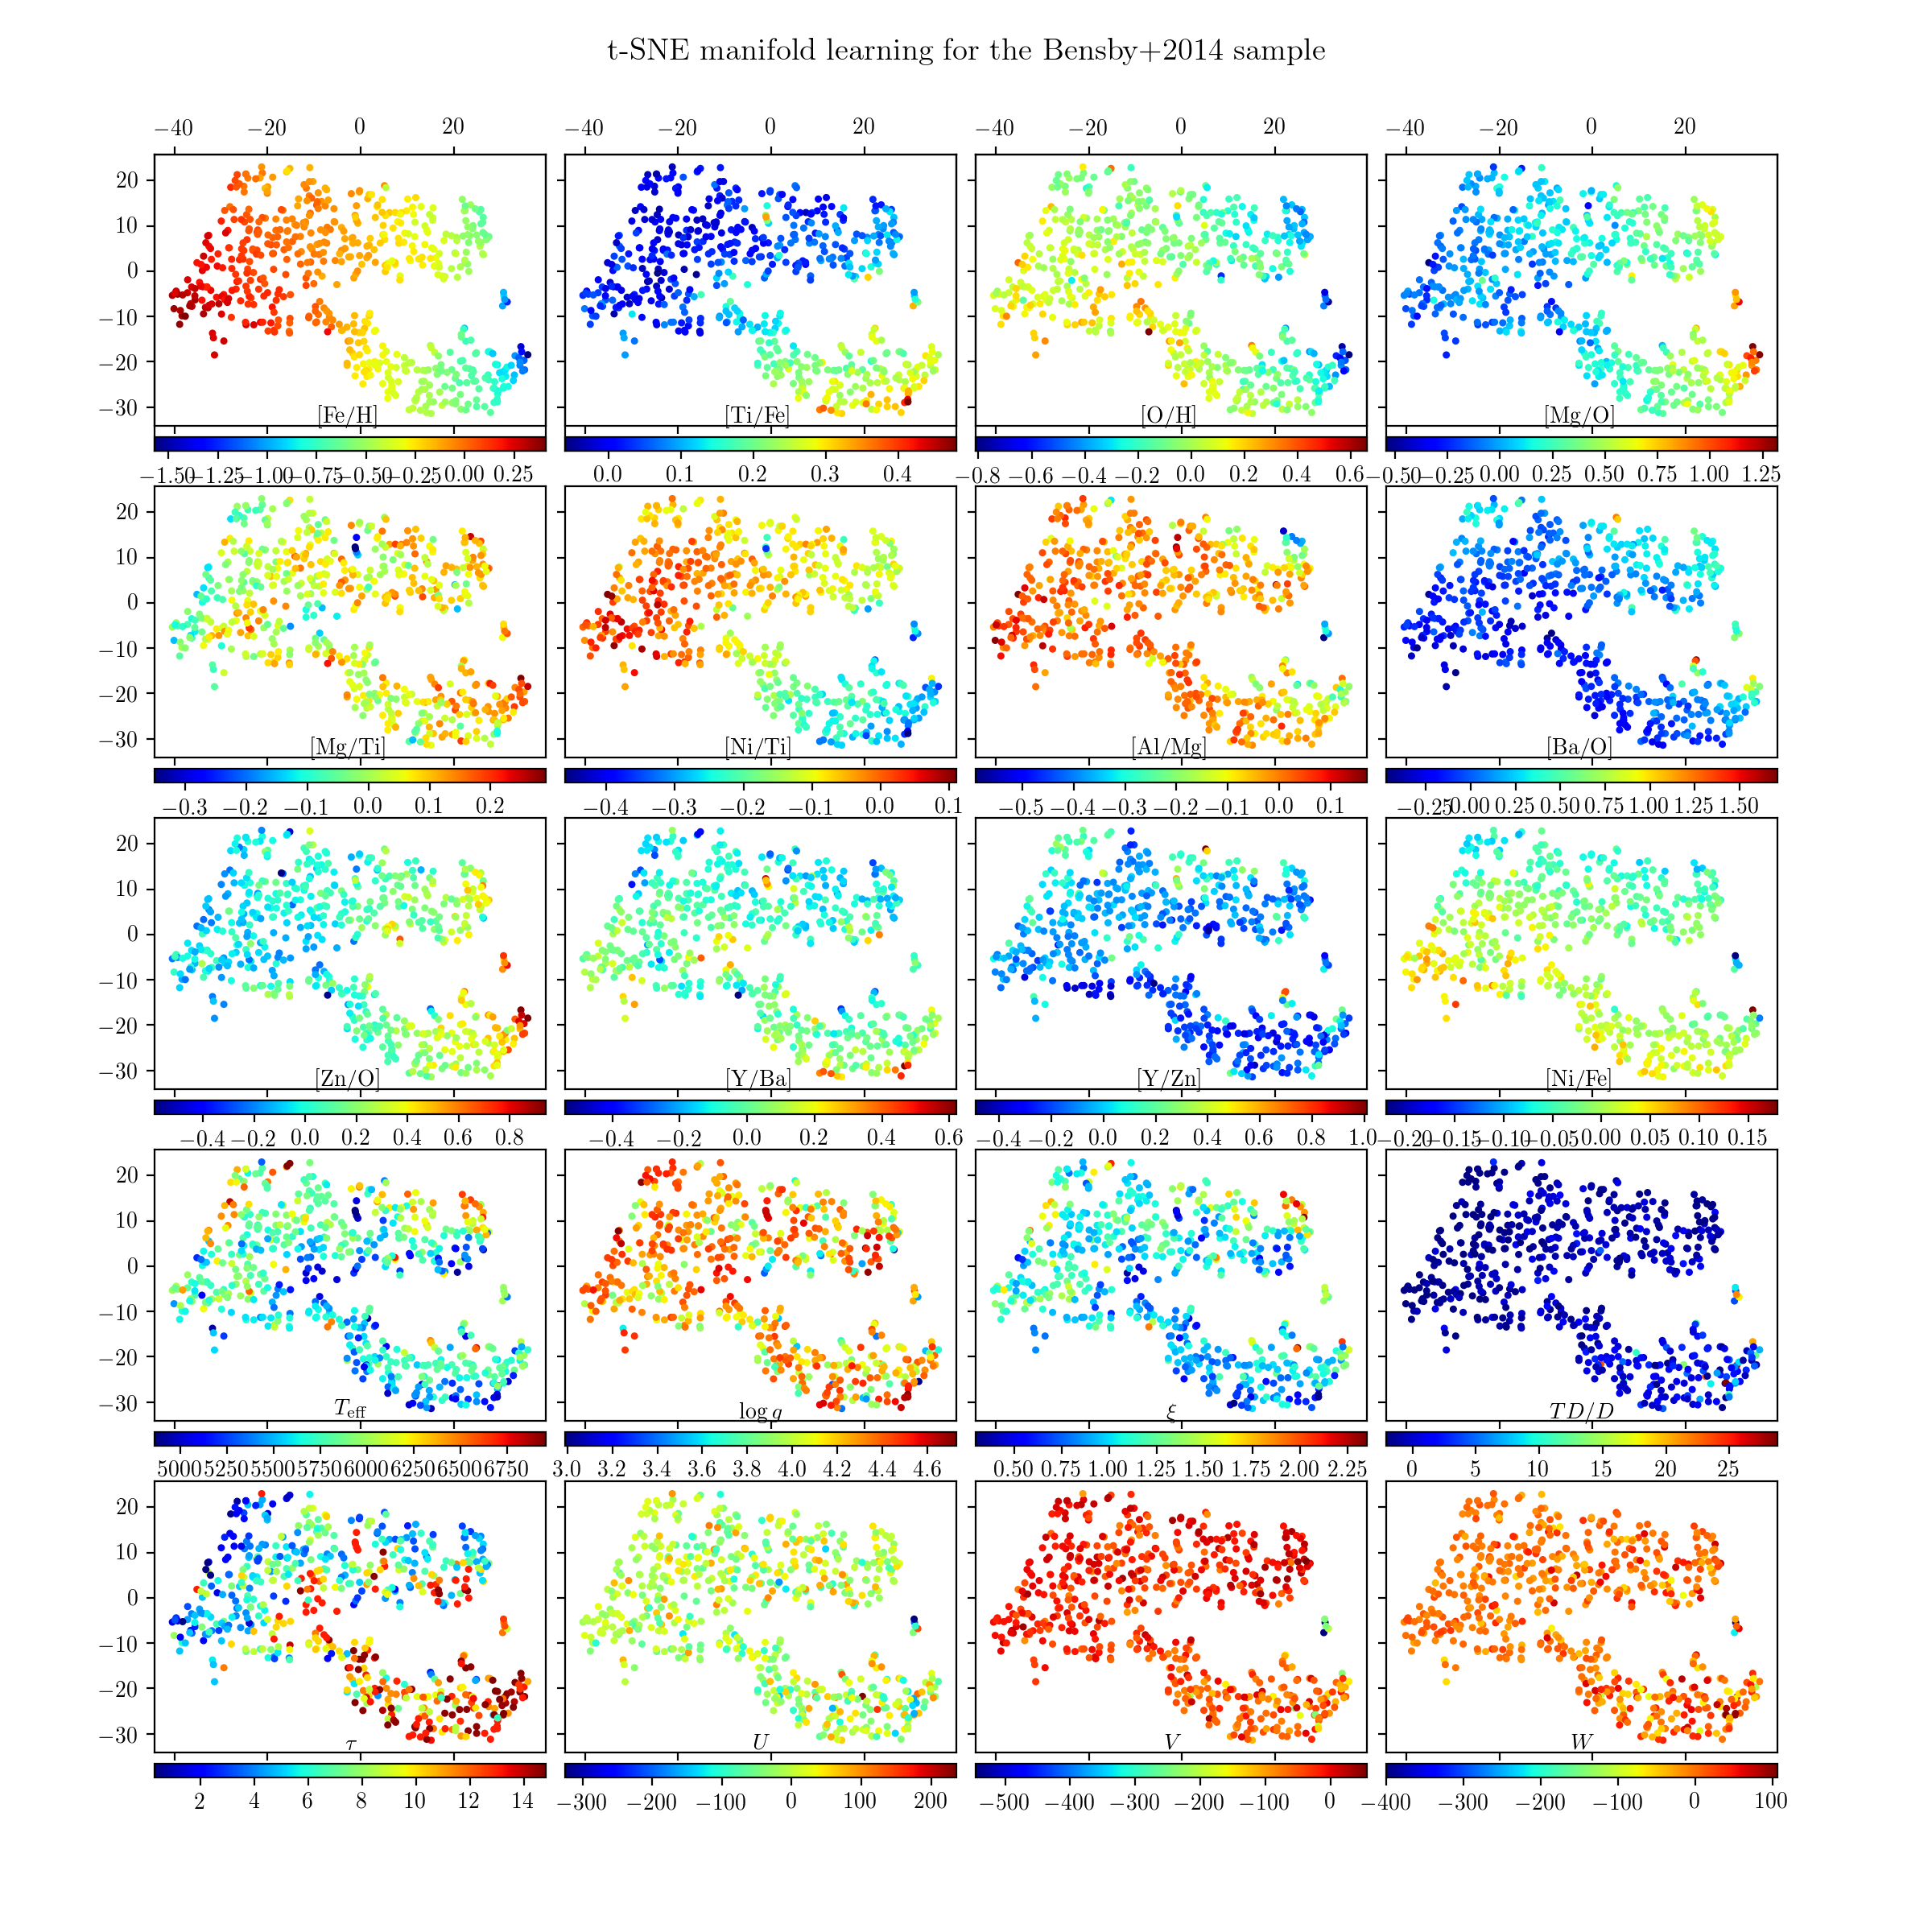
\includegraphics[width=0.99\textwidth]{Bensby2014_tsne_plots15_rand0.png}
% \caption{t-SNE projection ($p=15$) of the \citet{Bensby2014} sample, colour-coded by chemical abundances (top three rows), stellar atmospheric parameters (fourth row), thick-to-disc probability (fourth row, last panel), age (fifth row, first panel) and UVW velocities (fifth row). We note that only [Fe/H] and the [X/Fe] ratios were used as input for the t-SNE run. The distinct populations appearing in these diagrams are studied in detail in Fig. \ref{bensby2}.}
% \label{bensby1}
% \end{figure*}
% 
% \citet*{Bensby2014} studied the chemistry and kinematics of 714 FGK stars in the {\it Hipparcos} volume. Their sample was selected based on kinematic criteria that enabled the authors to explicitly study the metal-poor tail of the disc and its transition to the halo, as well as the metal-rich end of the thick disc. Using high-resolution optical spectroscopy, they report chemical abundances for the 13 elements O, Na, Mg, Al, Si, Ca, Ti, Cr, Fe, Ni, Zn, Y and Ba. This high number of measured abundances, in conjunction with the high precision of the measurements and the reasonable sample size, makes the Bensby sample an ideal test case for our machine-learning algorithm. However, since t-SNE cannot cope with missing data, we select only the 600 stars for which all these abundances were available for our analysis, which results in a lower metallicity limit of [O/H] $>-0.8$. Since our main interest here is in the chemical substructure of the disc, this requirement does not hinder our analysis. 
% \begin{itemize}
%  \item the absence of kinematic selection biases: The HARPS sample initially served to detect and characterise exoplanets and may therefore contain some metallicity-related selection bias; however, e.g. \citet{Anders2014} have shown that the HARPS metallicity distribution (MDF) matches the MDF of high-quality local ($d<1$ kpc) APOGEE red-giant stars that could be considered less chemically biased. In contrast to the \citet{Bensby2014} sample, it was not targeted based on kinematic priors.
%  \item the availability of different abundances: O, Na, V, Cr, Co and Ni are only available for the Bensby sample, while Sr, Zr and Ce are only available for the HARPS sample. Carbon estimates are available from a previous study \citep{Suarez-Andres2017}, but since they are based on previous stellar parameter estimates, we decided to only use them in the interpretation. We also did not use Nd and Eu, and the O estimates from \citet{BertrandeLis2015} in the t-SNE run, because they were only available for about half of the sample (stars with the highest signal-to-noise ratios). We do, however, use the Nd and Eu results in the interpretation, whenever they are available.
% \end{itemize}

% 
% \begin{figure*}\centering
%  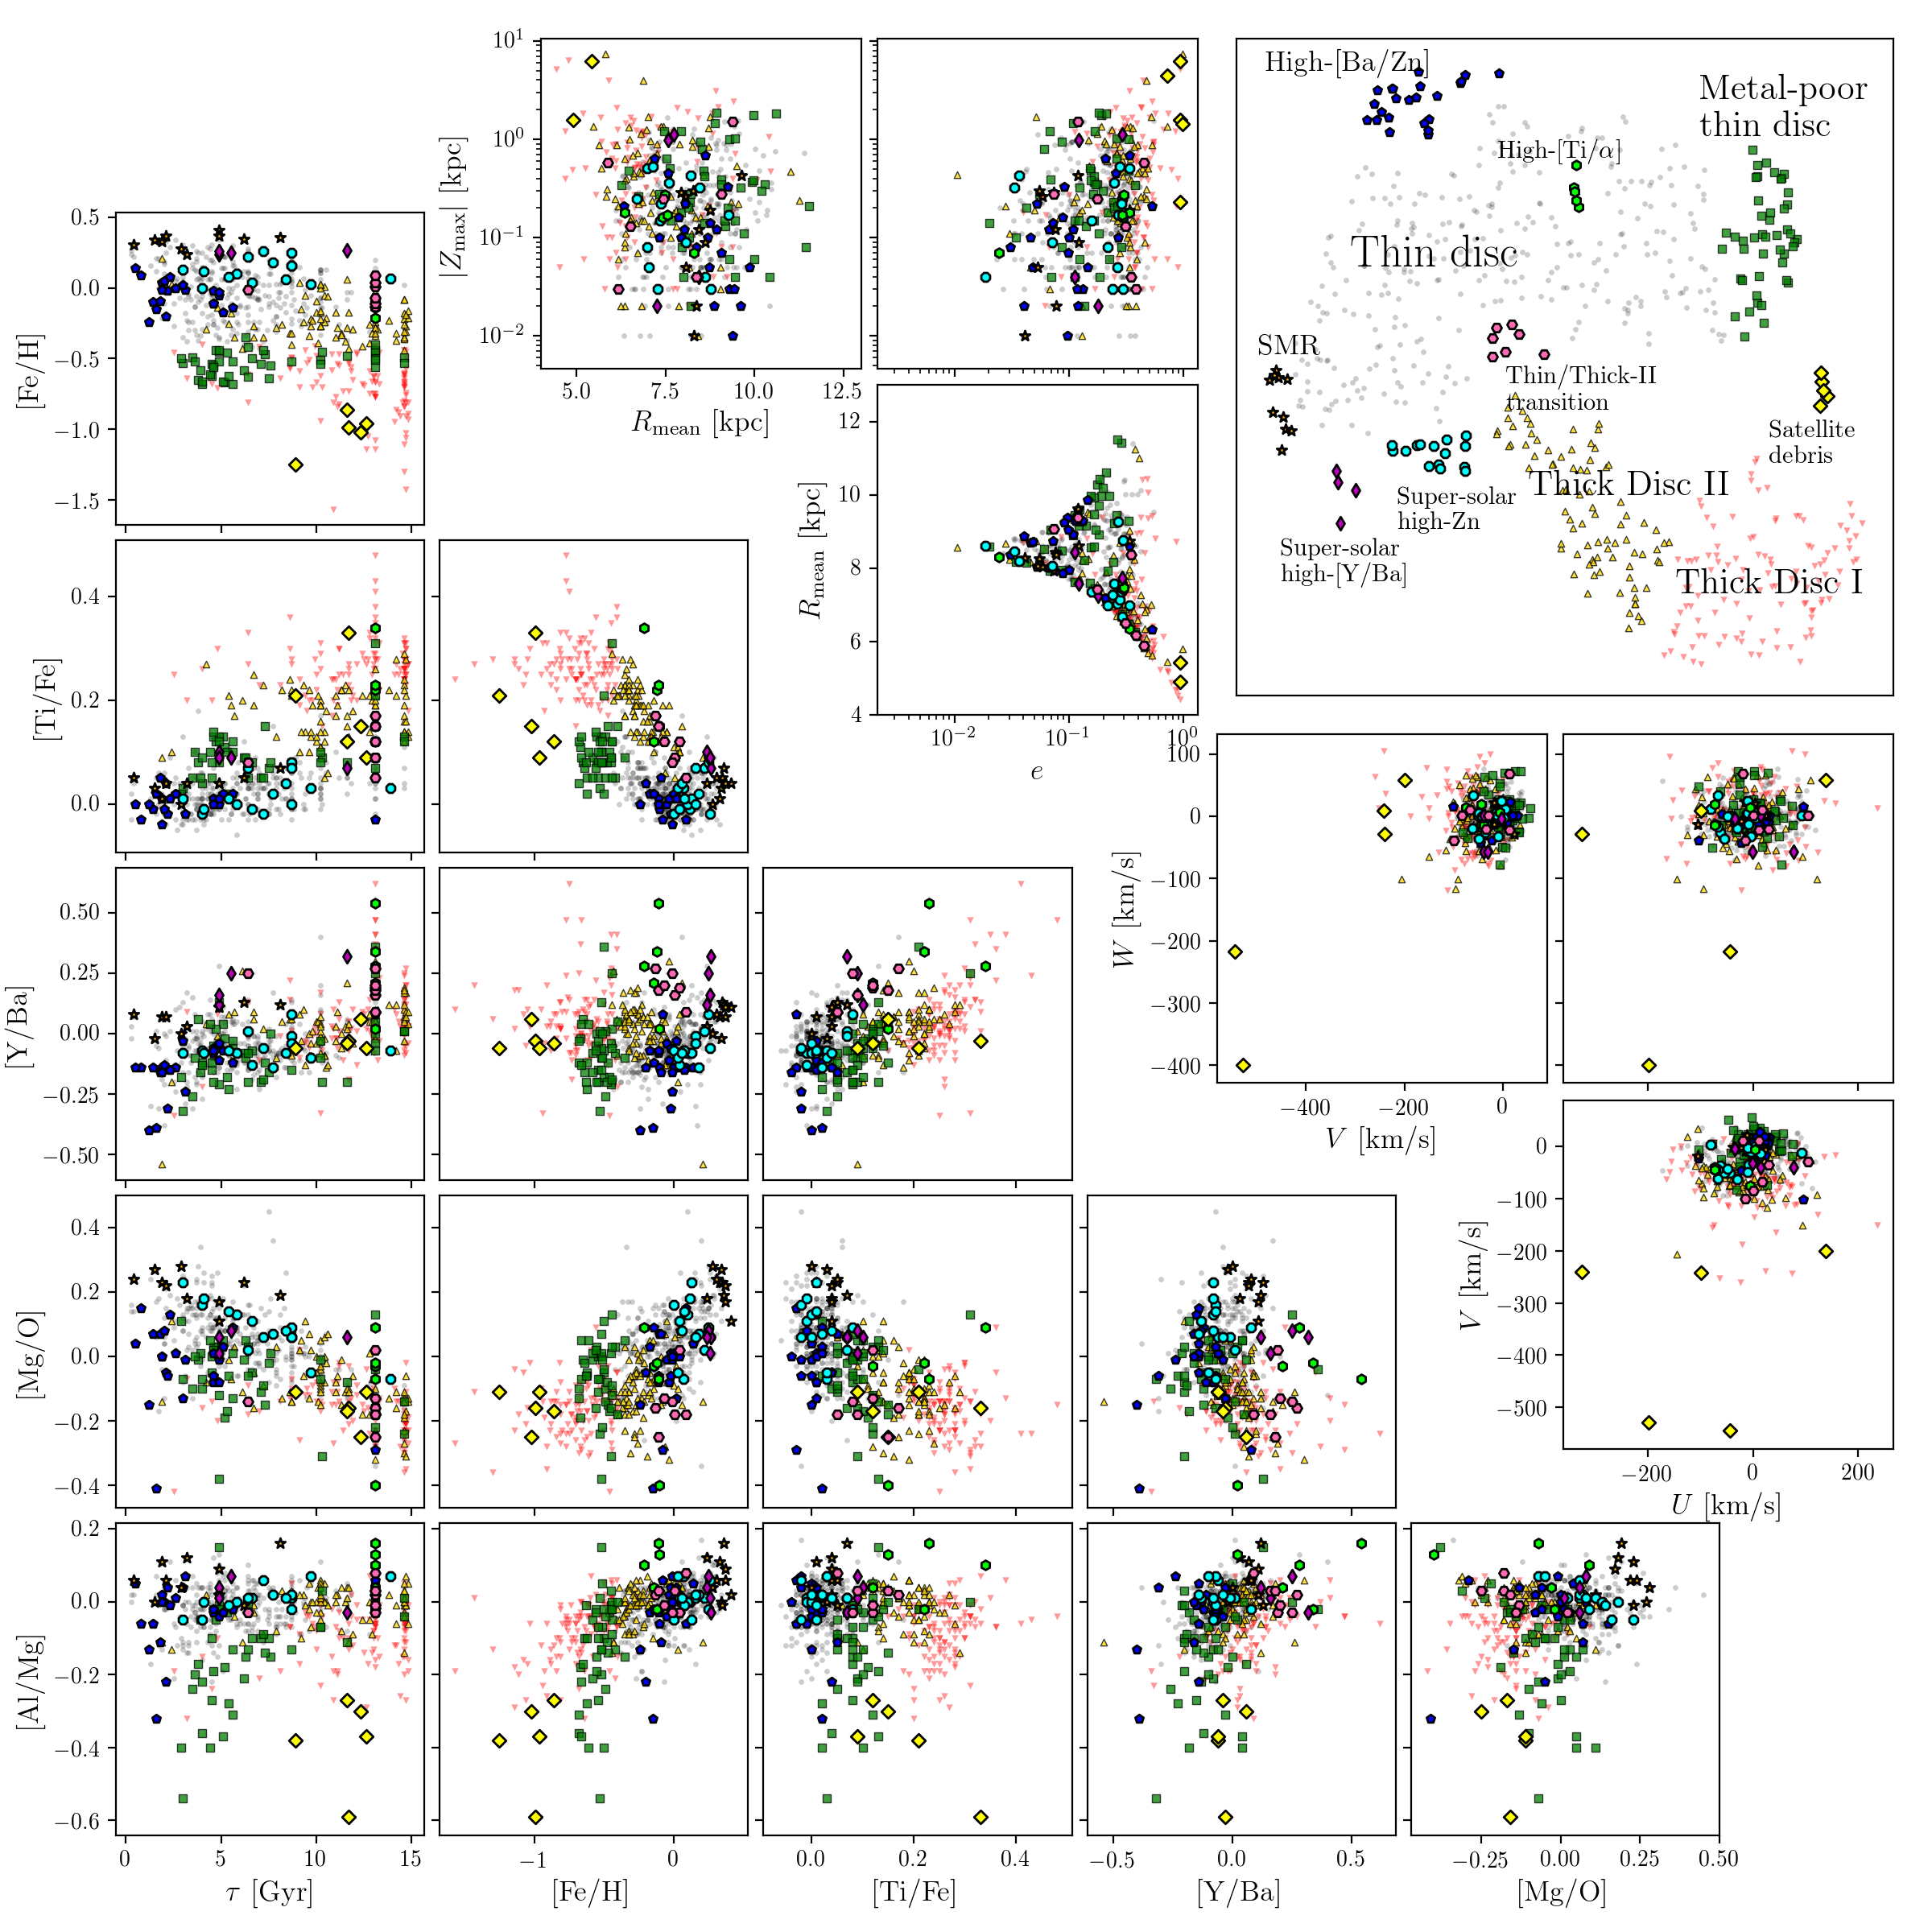
\includegraphics[width=0.99\textwidth]{bensby2014_tsne-summary-plot.png}
% \caption{The chemo-chrono-kinematic distribution of t-SNE-selected subsamples of the \citet{DelgadoMena2017} sample, in a similar style as Fig. \ref{harps2}.}
% \label{bensby2}
% \end{figure*}
% 
% \begin{figure*}\centering
%  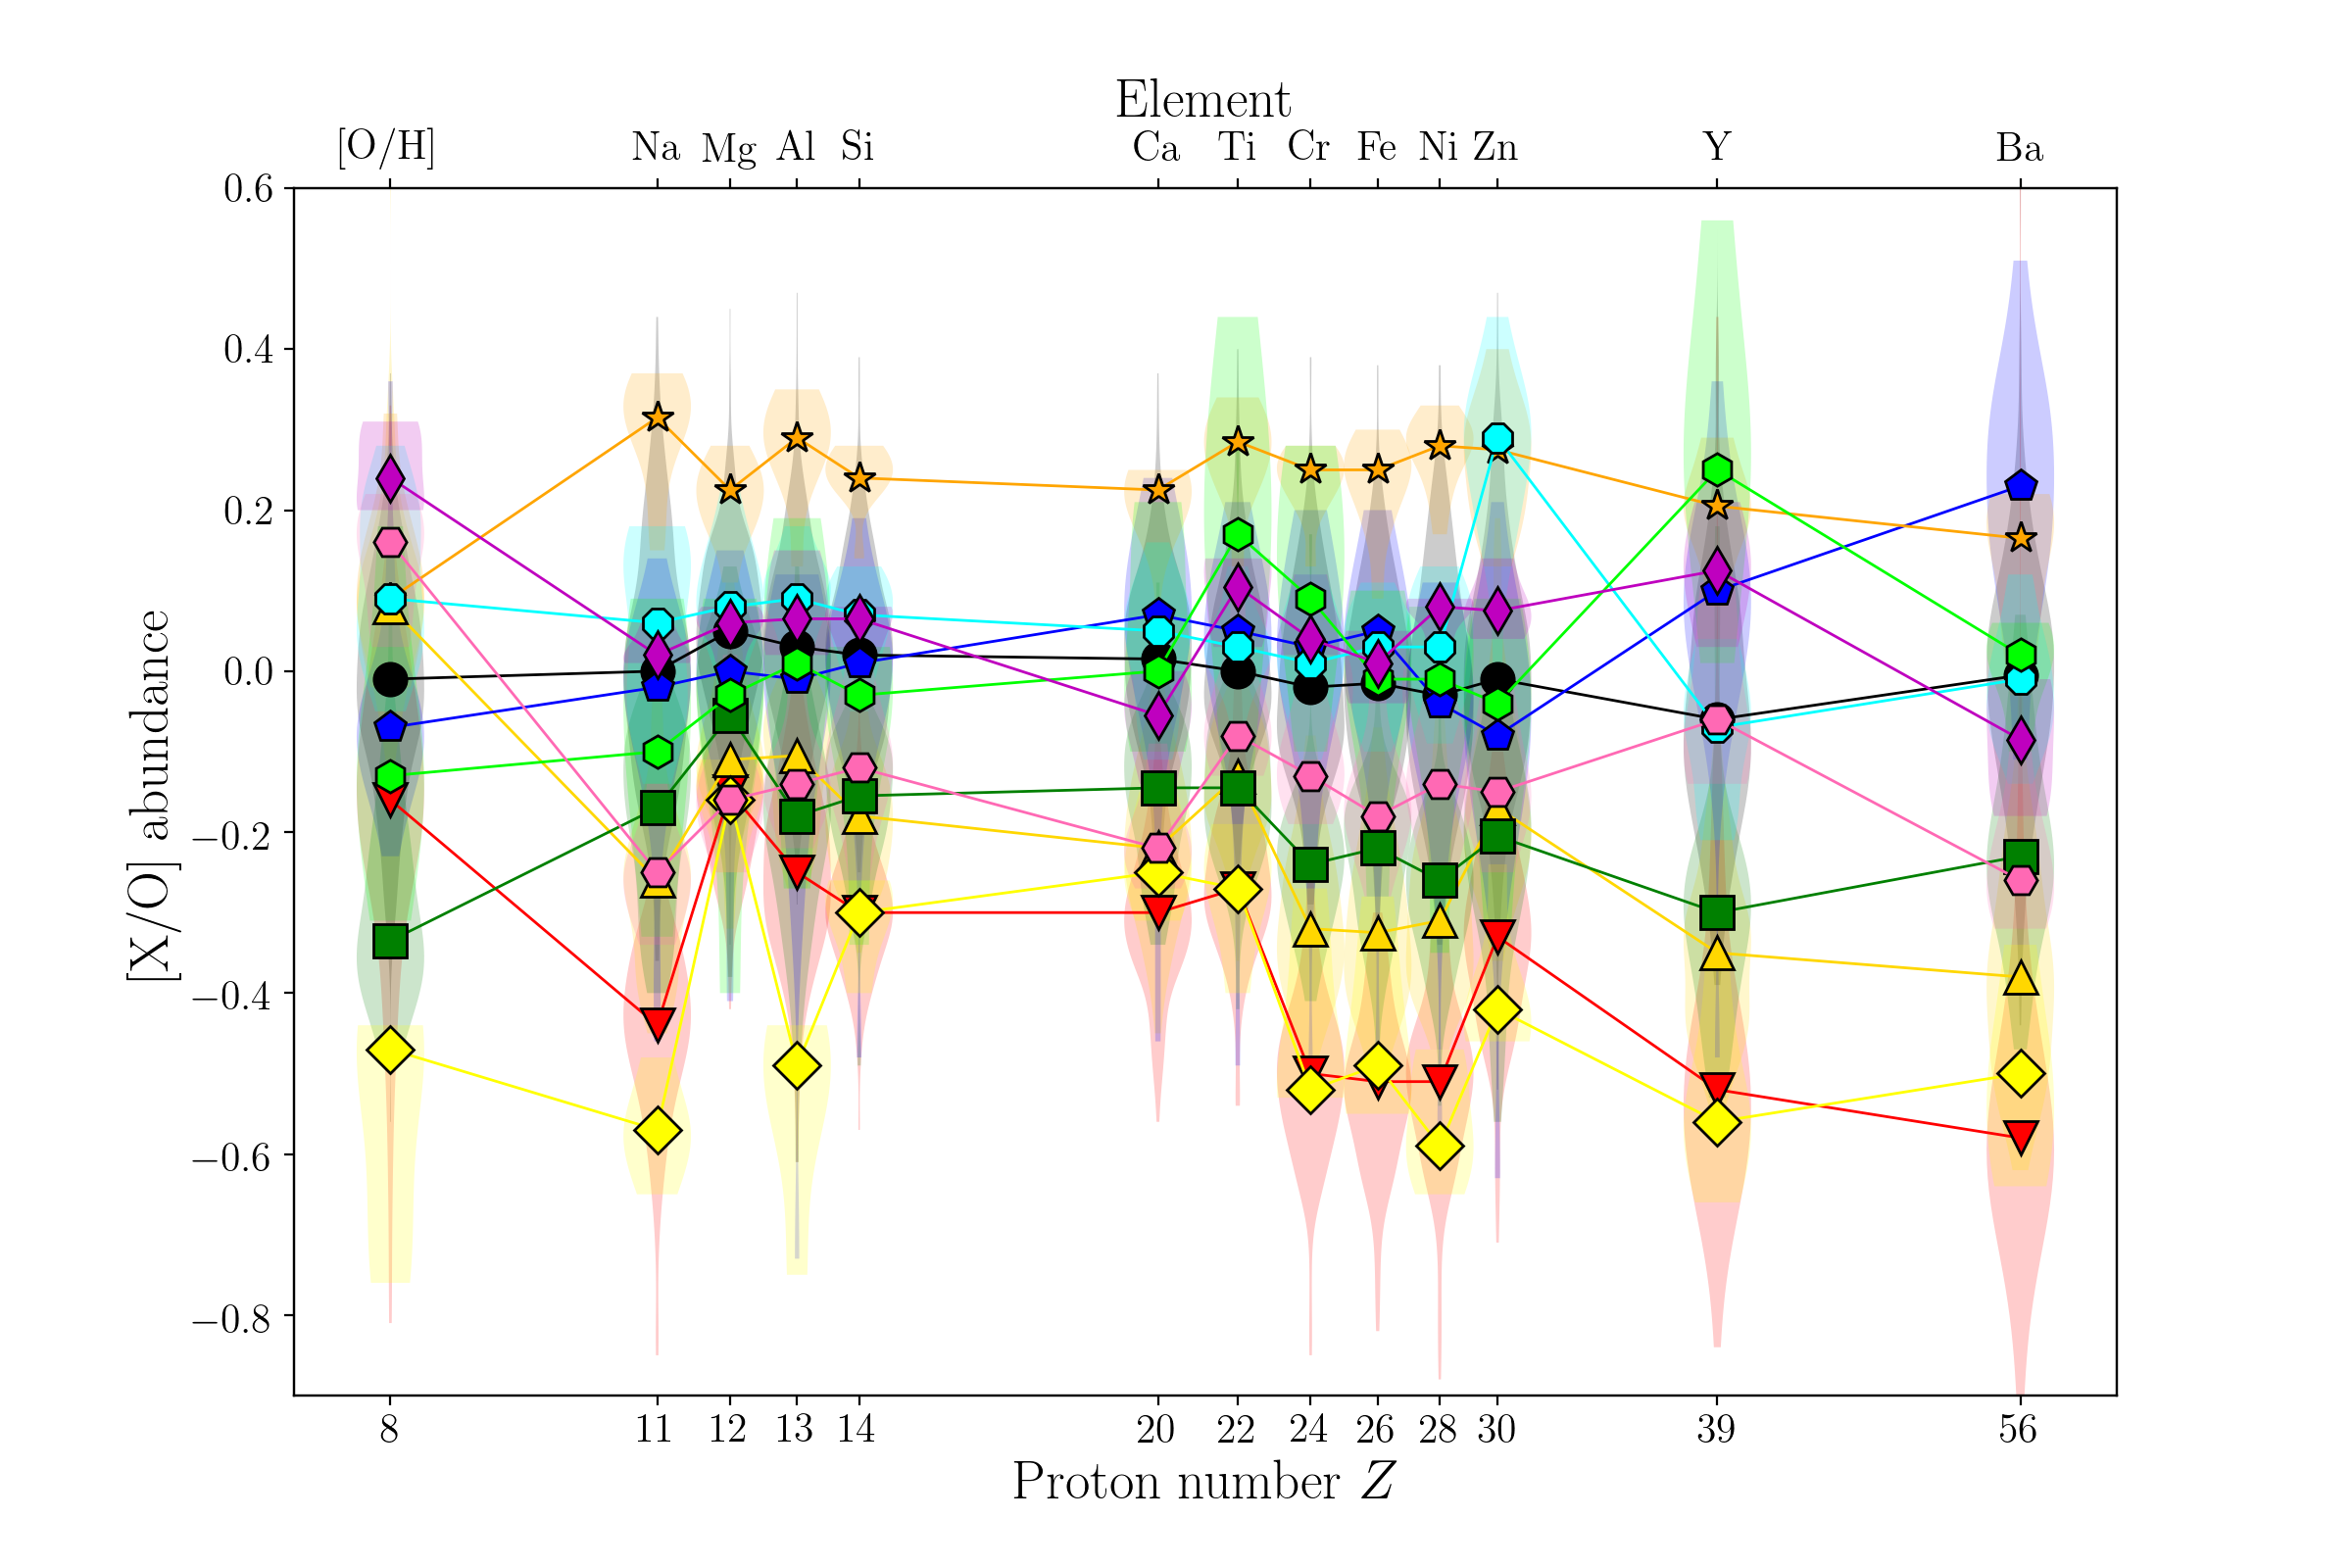
\includegraphics[width=0.99\textwidth]{bensby2014_tsne_abundances-relto-O.png}
% \caption{Chemical-abundance patterns relative to oxygen for the t-SNE-selected subsamples of the \citet{Bensby2014} survey (colours and symbols as in Fig. \ref{bensby2}). For visibility, we show only the median abundance ratios of each group.}
% \label{bensby3}
% \end{figure*}
% 
% Since t-SNE is a highly non-linear projection method, and since sample and its abundance determination method differ significantly from the stars studied by \citet{Bensby2014}, the overall morphologies of the t-SNE maps in Figs. \ref{bensby1} and \ref{harps1} are also expected to be dissimilar. While this is indeed the case, there are some features that appear in both maps, and can therefore be suggested to be generic properties of the solar-neighbourhood abundance space:
% 
% In Fig. \ref{bensby2} we identify some of the substructures that appear in Fig. \ref{bensby1}, and discuss them below. In addition, Fig. \ref{bensby3} shows the corresponding [X/O] abundance trends versus proton number, for each of the subpopulations defined in Fig. \ref{bensby2}.
% 
% {\it The thin-thick discontinuity}: We find a clear and obvious dichotomy of thin and thick disc in the t-SNE diagram (upper left vs. lower right) that remains robust for different choices of the perplexity value. Primarily, this means that the chemical patterns of thin and thick disc are indeed distinct, and can be disentangled by high-resolution spectroscopy. Secondly, our analysis of the full chemical information results in a much more accurate division of the chemically-thin and thick populations. Indeed, if one only relies on one diagnostic, such as the [Ti/Fe] vs. [Fe/H] diagram \citep{Bensby2014}, several stars (e.g. thin-disc stars that have an unusual [Ti/$\alpha$] ratio -- limegreen hexagons in Fig. \ref{bensby2}, or low-[Fe/H] thin disc stars -- green squares) will be incorrectly identified as chemical thick disc. 
% 
% {\it h$\alpha$mr stars \& substructure in the thick disc:} \citet{Adibekyan2011} first discovered a clear discontinuity between the metal-poor and metal-rich $[\alpha$/Fe]-enhanced (or h$\alpha$mr) disc populations. In our t-SNE analysis of the \citet{Bensby2014} sample, similar to the original paper, we only see a hint of a difference between the two populations (dubbed Thick Disc I and II in Fig. \ref{bensby1}). The bimodality is better seen when slightly higher perplexity values are chosen ($p\sim 30$). Even if ages and/or kinematics are included as additional dimensions in the analysis, this picture does not change much. %Below we will show that the APOGEE-TGAS sample does reveal a clear distinction between the metal-rich and the metal-poor high-[$\alpha$/Fe] population, which is why we have also divided the Bensby sample in this manner (red vs. yellow triangles in Fig. \ref{bensby2}), along the apparent slight paucity of points in the t-SNE thick-disc sequence. This fact already indicates that, despite being derived from lower-resolution spectra, the APOGEE abundances might be better suited to disentangle chemically distinct stellar populations in the disc, most likely due to the availability of carbon and nitrogen abundances. 
% 
% {\it Thin-thick transition:} Most literature measurements agree that the high- and low-[$\alpha$/Fe] sequences in the [$\alpha$/Fe] vs. [Fe/H] diagram merge at super-solar metallicities (e.g. \citealt{Adibekyan2011, Anders2014, Hayden2015}). In other words, the upper metallicity limit of the high-[$\alpha$/Fe] or the h$\alpha$mr population is not yet firmly established. Out analysis shows that including the full chemistry information does not allow us to completely solve this question, since the border between thin-disc-like and thick-disc-like chemistry remains debatable in the t-SNE projection (e.g. the pink hexagons in Fig. \ref{bensby1} have intermediate characteristics between Thick Disc II and Thin disc). 
% 
% {\it Super-metal-rich stars:} SMR stars ([Fe/H] $>0.3$ -- the western-most stars in the t-SNE plane; orange stars in Fig. \ref{bensby2}) have only slightly different abundance patterns from the bulk of the thin disc stars (grey dots): they are slightly enhanced in [Y/Ba], for example, and slightly [Ti/Fe]-enhanced with respect to the thin disc, indicative of an origin in the inner Milky-Way disc. All but one have ages smaller than 5 Gyr, and are on cold orbits ($e<0.12$), which means that they have likely suffered from radial migration (see e.g. \citealt{Minchev2012, Vera-Ciro2014, Kordopatis2015, Grand2016, Anders2017}).
% 
% {\it The metal-poor thin disc:} The green squares in Fig. \ref{bensby2} correspond to the metal-poor thin disc ([Fe/H] $\sim-0.5$). Apart from metallicity, its main abundance differences with respect to the bulk of the chemical thin-disc population are: 1. a light elevation of [$\alpha$/Fe], as a consequence of the slower star-formation history in the outer disc, where this population is most likely to originate from (e.g. \citealt{Anders2014, Hayden2015}; see also kinematic diagnostics in Fig. \ref{bensby2}, especially the eccentricity-mean radius diagram), 2. a systematic deficiency in [Al/Mg], in conjunction with a rather striking correlation between [Al/Mg] and age for this group. A strong correlation between age and [Al/Mg] has recently been found in solar-metallicity solar twins \citep{Nissen2015, Nissen2016, TucciMaia2016, Nissen2017}. Here we find that this correlation persists for a broader range of stellar parameters, lower signal-to-noise ratios, and more uncertain age estimates, and appears much stronger for the metal-poor thin-disc stars. 
% 
% {\it Other potential groups and substructures in the thin disc:} In Fig. \ref{bensby2} we also highlight several other smaller groups of stars that can be viewed as sub-populations of the chemical thin disc, but are peculiar in some respect. These are: a) a group of stars with high zinc abundances (cyan octagons), but otherwise typical thin-disc-like abundances (see Fig. \ref{bensby3}); b) a group of four SMR stars ([Fe/H] $\approx0.2$, [O/H] $\approx0.25$) with slightly elevated [Y/Ba], [Ti/Fe], and [O/Mg] abundance ratios (with respect to stars of similar metallicities); c) a group of slightly s-process-enhanced solar-metallicity stars (most notably enhanced in [Ba/Zn]; blue pentagons); and a group of five stars with enhanced [Ti/$\alpha$], [Al/Mg], and [Y/Ba] ratios (limegreen hexagons). 
% A detailed discussion of these objects is likely premature, but our results, in conjunction with the cluster experiment of \citet{Kos2017}, already demonstrate the potential of t-SNE for chemical-tagging studies. 
% 
% {\it Satellite debris:} Another observation of Fig. \ref{bensby2} is that our method clearly singles out a small group of five stars with dwarf-galaxy or globular-cluster-like abundance pattern (some more were lost due to the abundance quality cut). These five stars (HIP 34285, HIP 55592, HIP 58962, HIP 61802, HIP 90261; yellow diamonds in Fig. \ref{bensby2}) are all on highly eccentric orbits, have low [Al/Mg] and high [Zn/O] abundances, and four of them are [Ti/Fe]-poor, placing them in the typical dwarf-galaxy regime.
% 
% 
% 
% %%%%%%%%%%%%%%%%%%%%%%%%%%%%%%%%%%%%%%%%%%%%%%%
% \section{Caveats and possible improvements}\label{caveats}
% %%%%%%%%%%%%%%%%%%%%%%%%%%%%%%%%%%%%%%%%%%%%%%%
% 
% \subsection{Choosing the abundance space}
% 
% The t-SNE results for the \citet{Bensby2014} dataset are shown in Fig. \ref{perplexitytest}, for a range of perplexity values and different input. Following the recommendations of \citet{vanderMaaten2008} and \citet{Wattenberg2016}, we use this figure to choose the optimal perplexity value for each dataset (yellow-highlighted panels). In the following subsections, we analyse these results in detail.
% 
% \begin{figure}\centering
%  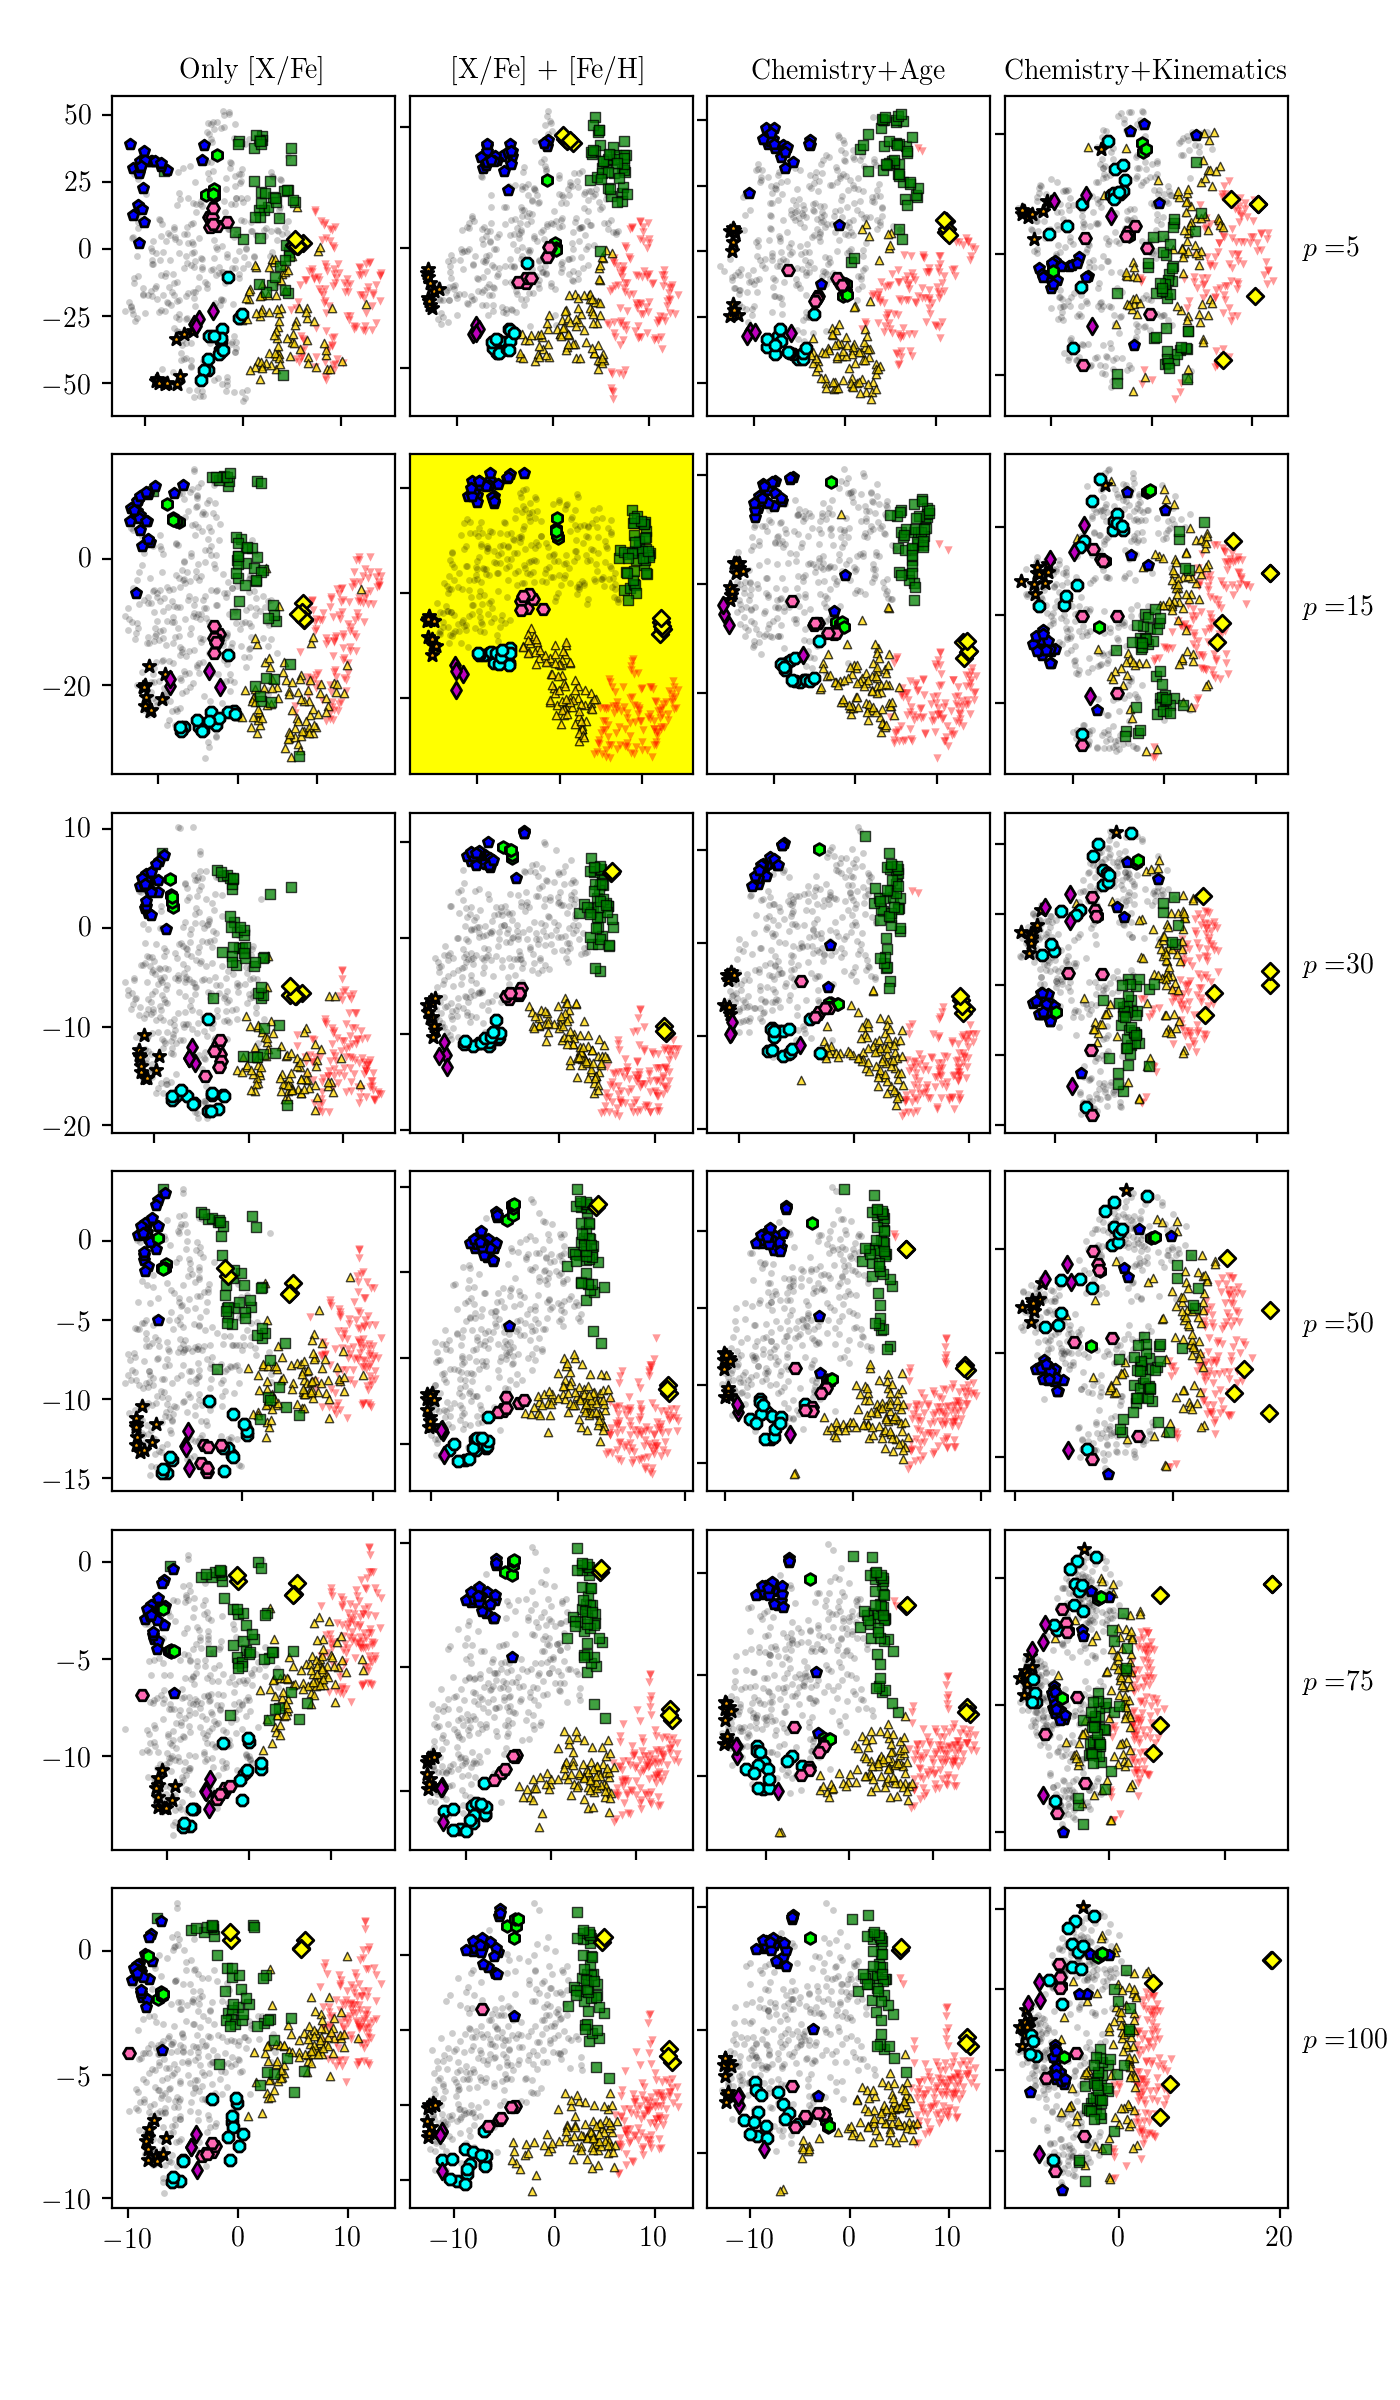
\includegraphics[width=0.49\textwidth]{bensby-tSNE_perplexitytest_withsubsets.png}
% \caption{t-SNE representations of the chrono-chemo-kinematics space spanned by the \citet{Bensby2014} sample. }
% \label{perplexitytest}
% \end{figure}
% 
% 
% 
% \subsection{Residual trends with stellar parameters}
% \subsection{The effect of adding age and kinematics to the analysis}

%%%%%%%%%%%%%%%%%%%%%%%%%%%%%%%%%%%%%%%%%%%%%%%
\section{Conclusions}\label{conclusions}
%%%%%%%%%%%%%%%%%%%%%%%%%%%%%%%%%%%%%%%%%%%%%%%

YES WE CAN use t-SNE to better define subpopulations in abundance space. However, the non-parametric non-linear behaviour of the technique makes it difficult to estimate the significance of found subgroups or clusters. The method could, however, be coupled to a genuine cluster finding algorithm.

Potential for weak chemical tagging demonstrated in this paper; the viability of t-SNE for strong chemical tagging (finding dispersed members of open clusters) is still not completely clear, but see \citet{Kos2017}.

It is better to confine the analysis to narrow regions in atmospheric-parameter space to avoid spurious abundance trends induced by differences in atmospheric parameters. 



\bibliographystyle{aa}
\bibliography{FA_library}


\begin{acknowledgements}
FA would like to thank Elisa Delgado-Mena for sharing the re-reduced HARPS-GTO data, and Guillaume Guiglion, Katia Cunha, Paula Jofr\'e, Bertrand Lemasle and the other participants of the IAU symposium 334 in Potsdam, as well as David W. Hogg, for their encouragement and critical thoughts. 

\end{acknowledgements}

%-------------------------------------------------------------------
\end{document}
